\documentclass[12pt]{article}

\usepackage{dcolumn}
\usepackage{rotating}

\begin{document}

% Figures
\begin{figure}
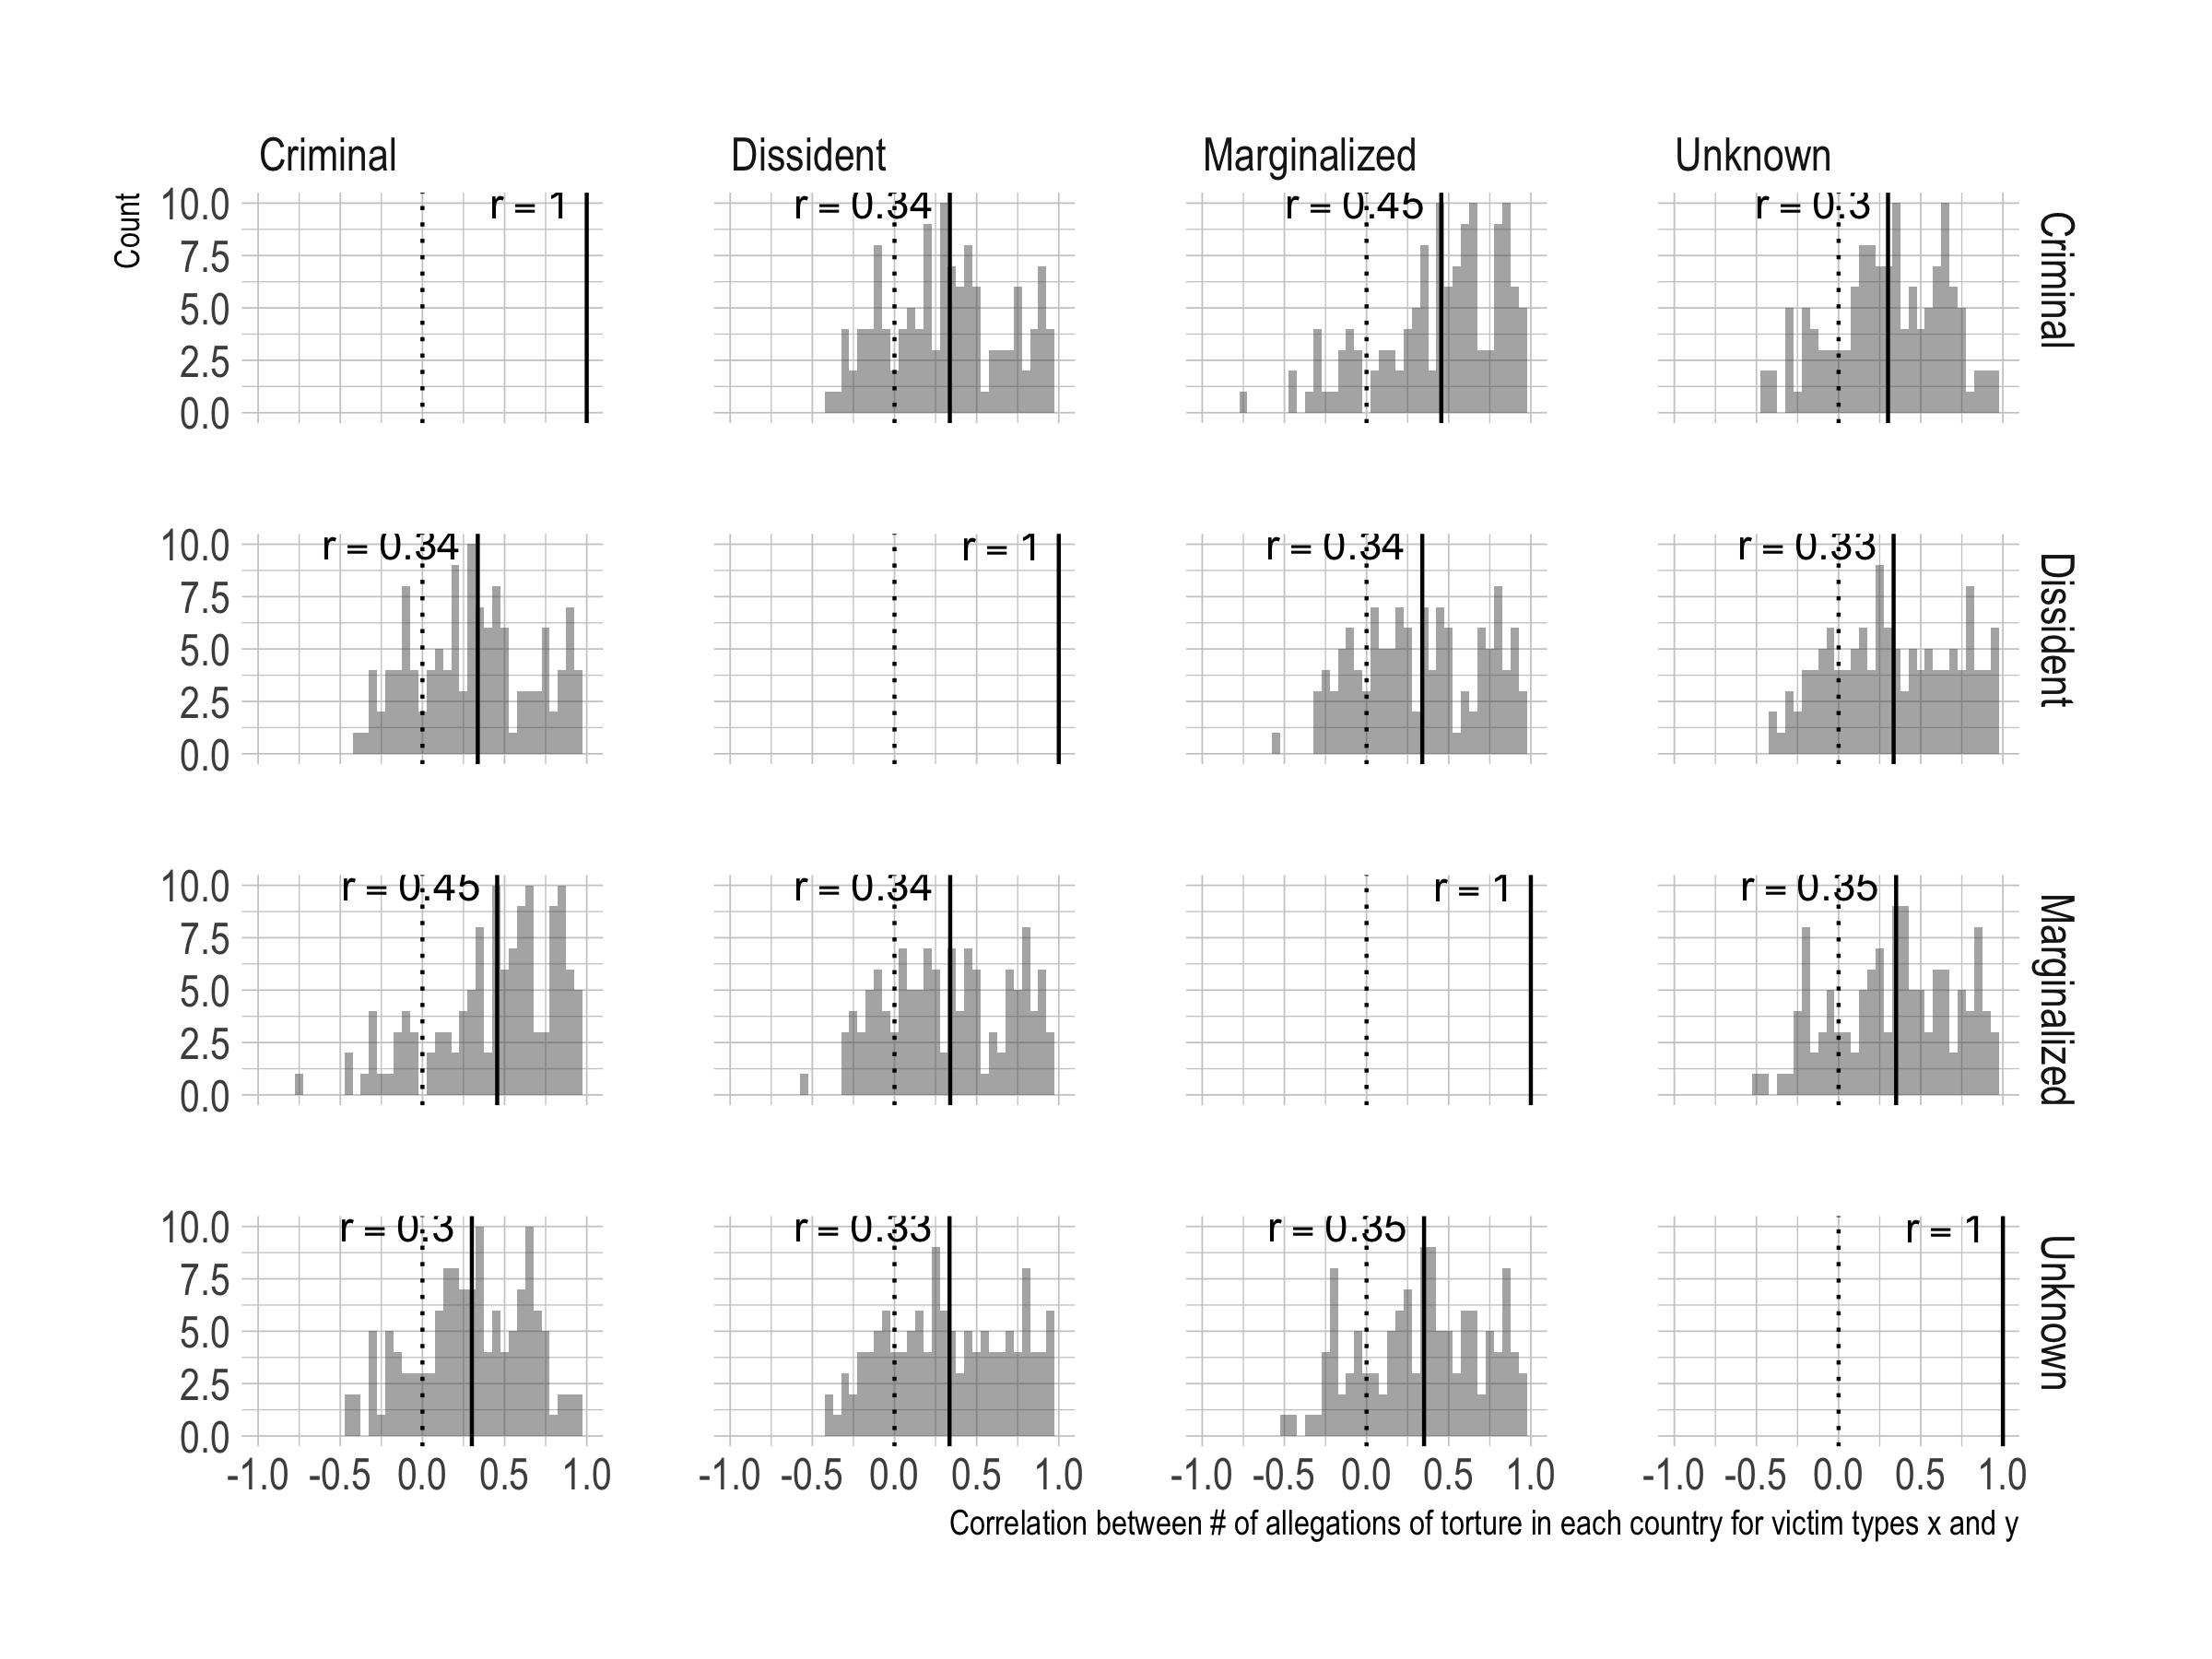
\includegraphics[width=.9\textwidth]{../output/figures/allegations-by-victim-pairwise-correlations.png}
\end{figure}

\begin{figure}
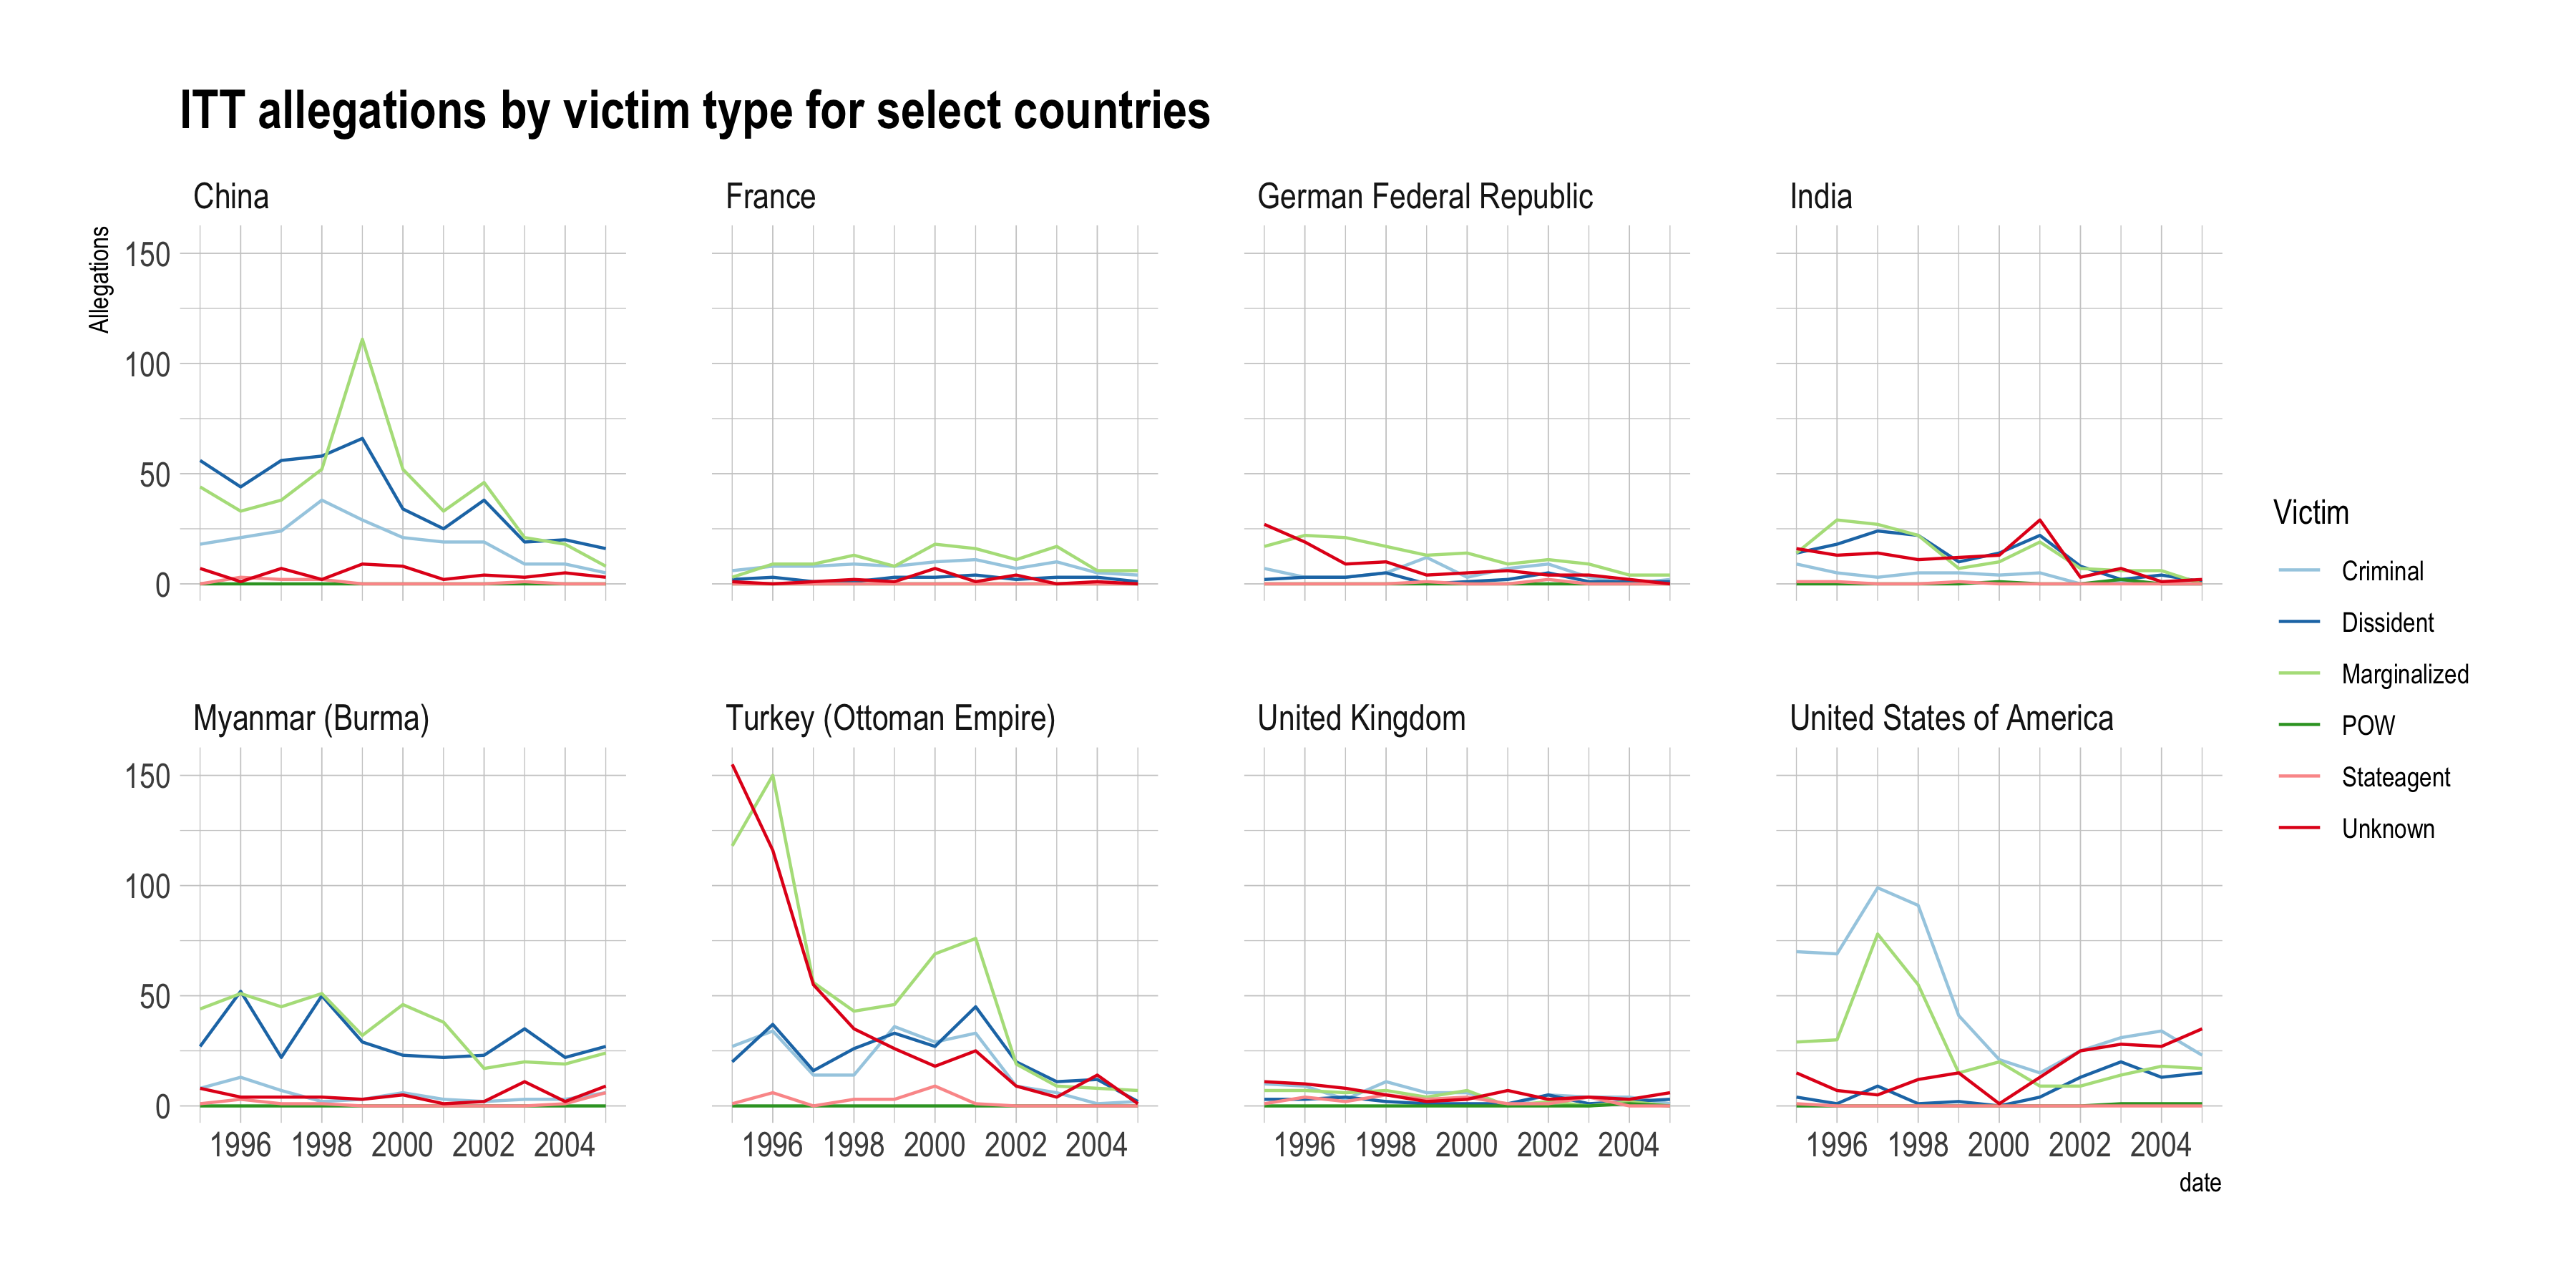
\includegraphics[width=.9\textwidth]{../output/figures/selected-allegation-counts.png}
\end{figure}

\begin{figure}
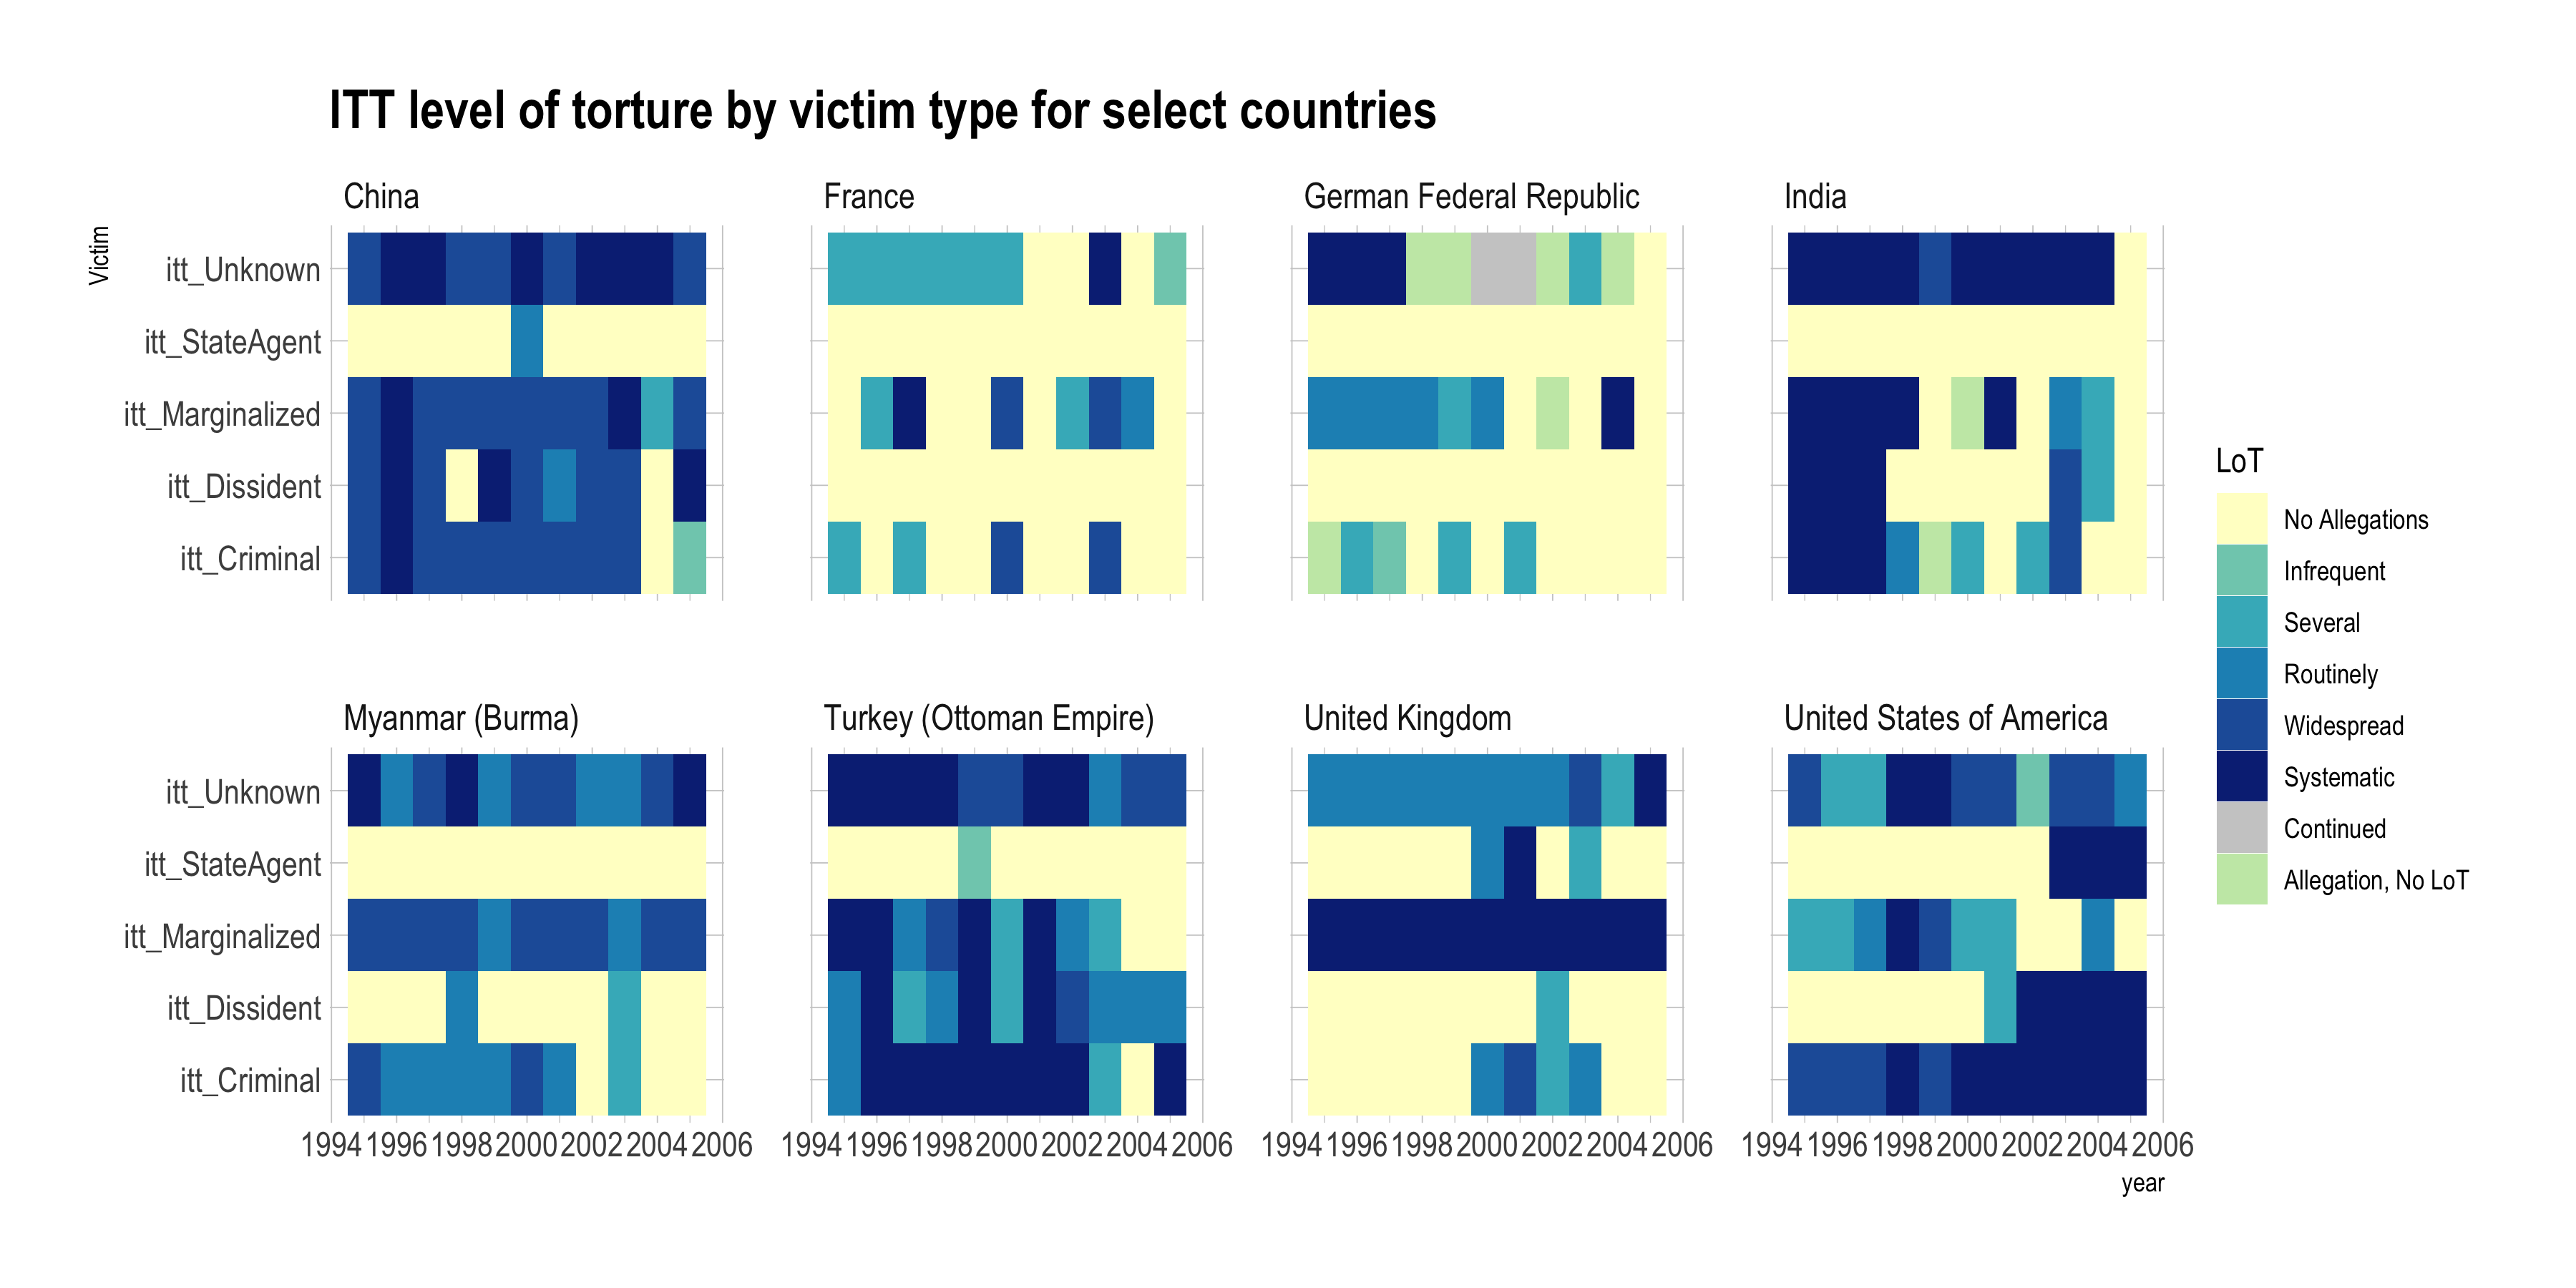
\includegraphics[width=.9\textwidth]{../output/figures/selected-levels-of-torture.png}
\end{figure}

\begin{figure}
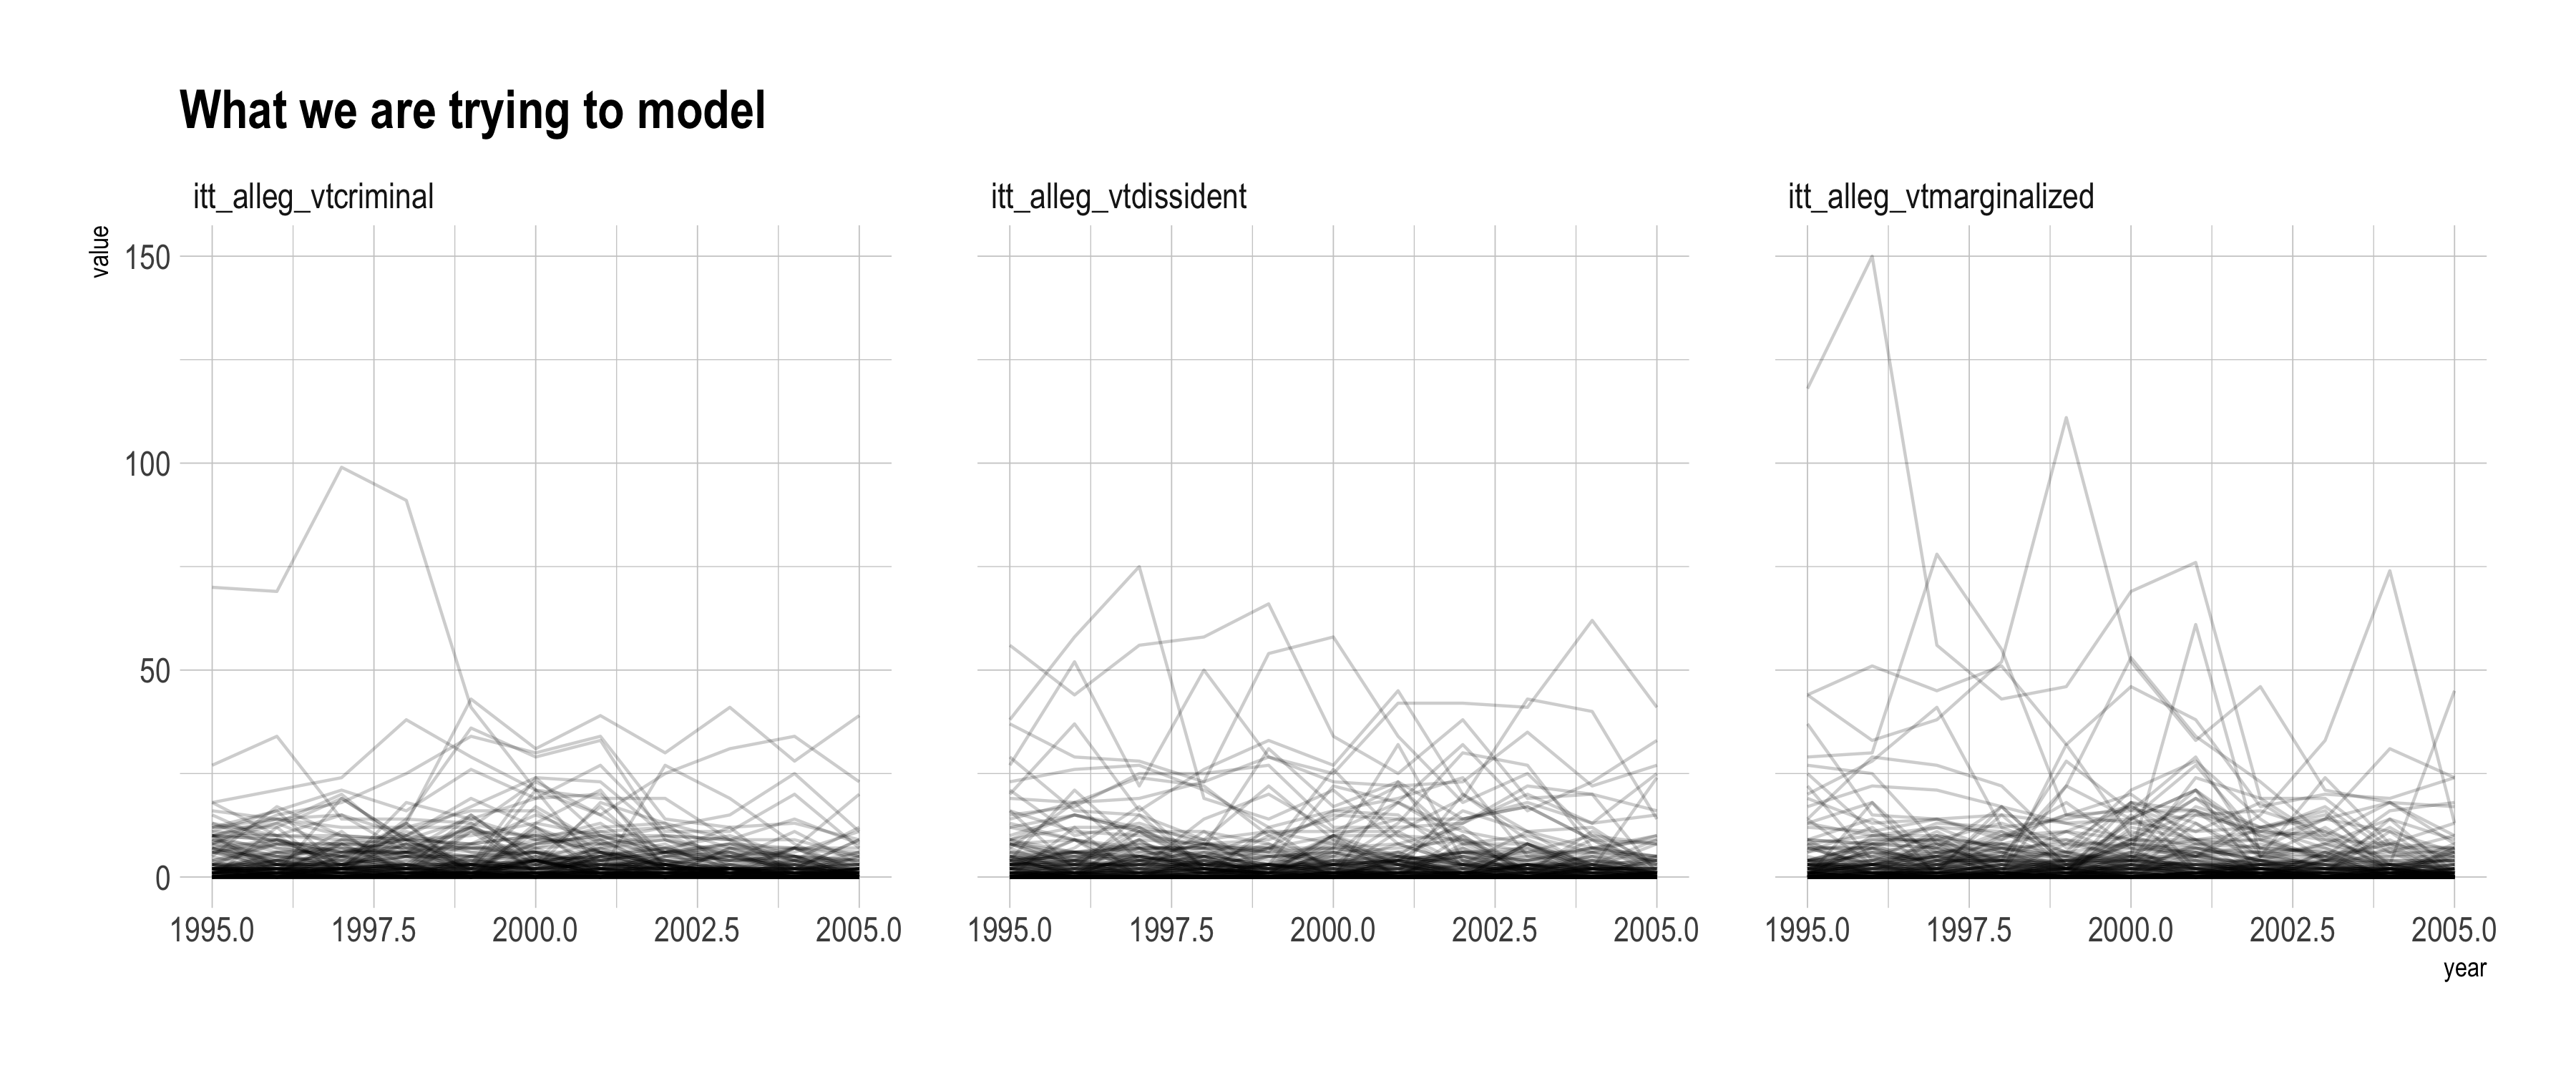
\includegraphics[width=.9\textwidth]{../output/figures/outcome-time-series.png}
\end{figure}

\begin{figure}
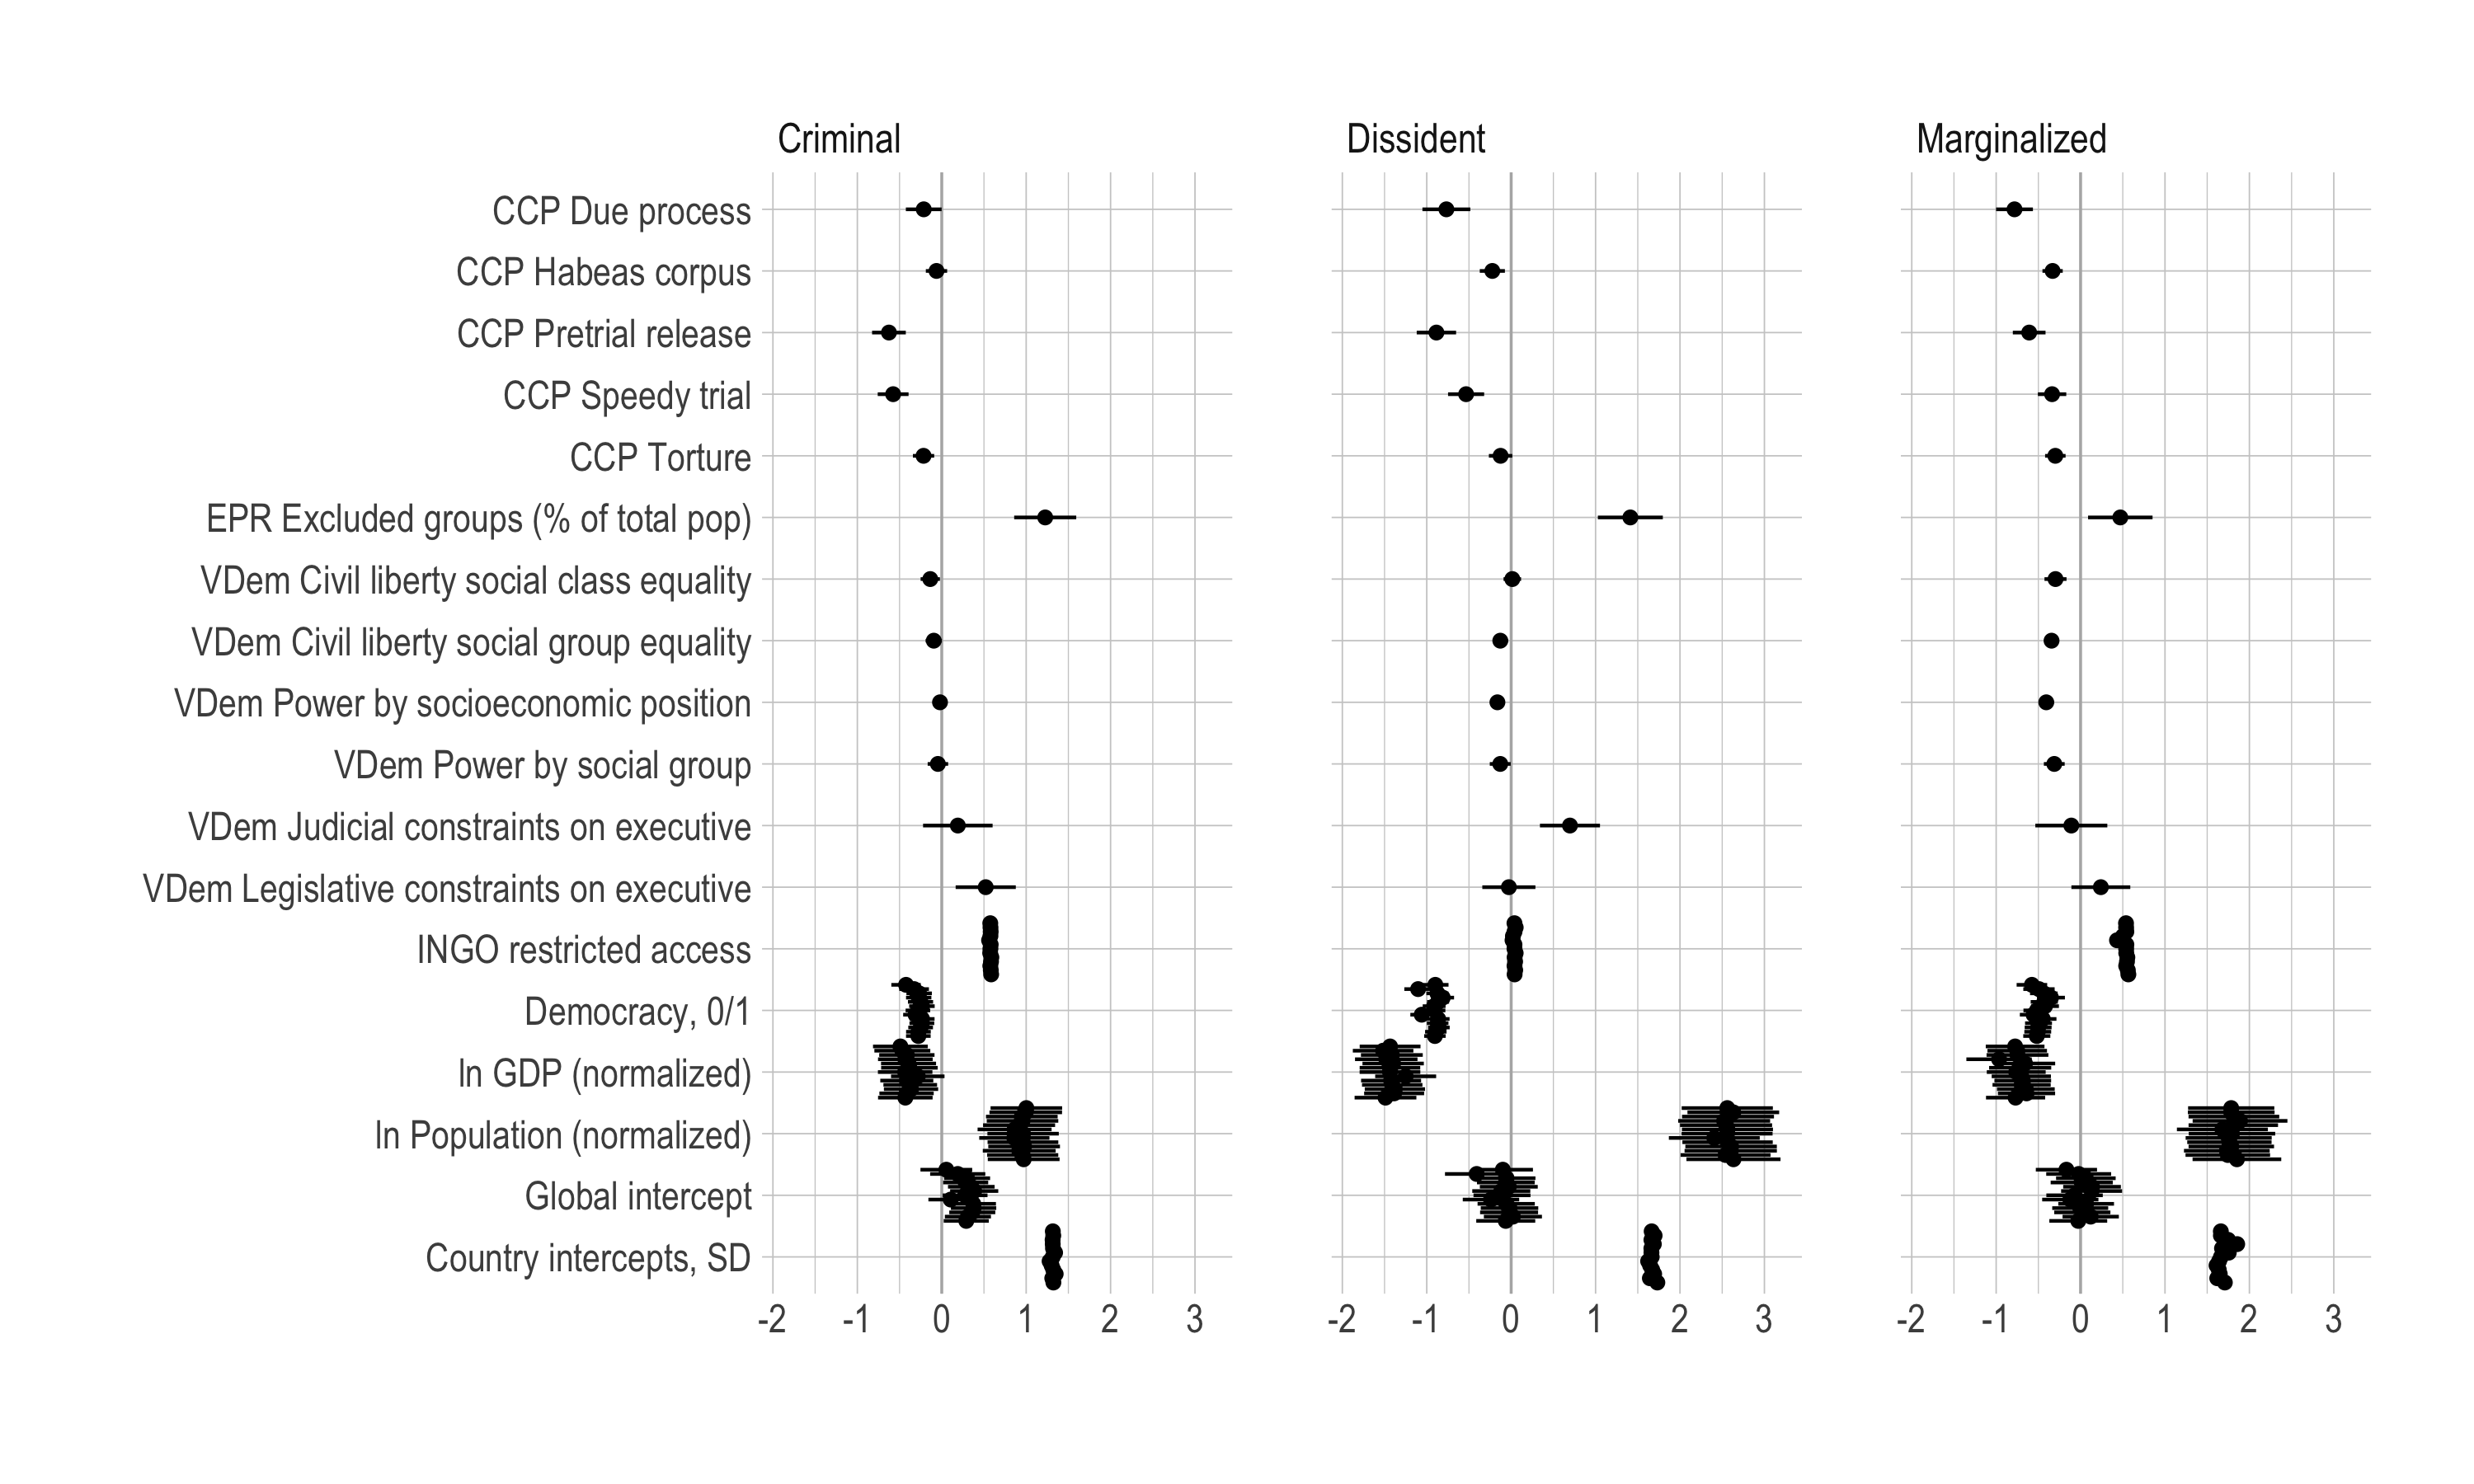
\includegraphics[width=.9\textwidth]{../output/figures/model-coefs.png}
\end{figure}

\begin{figure}
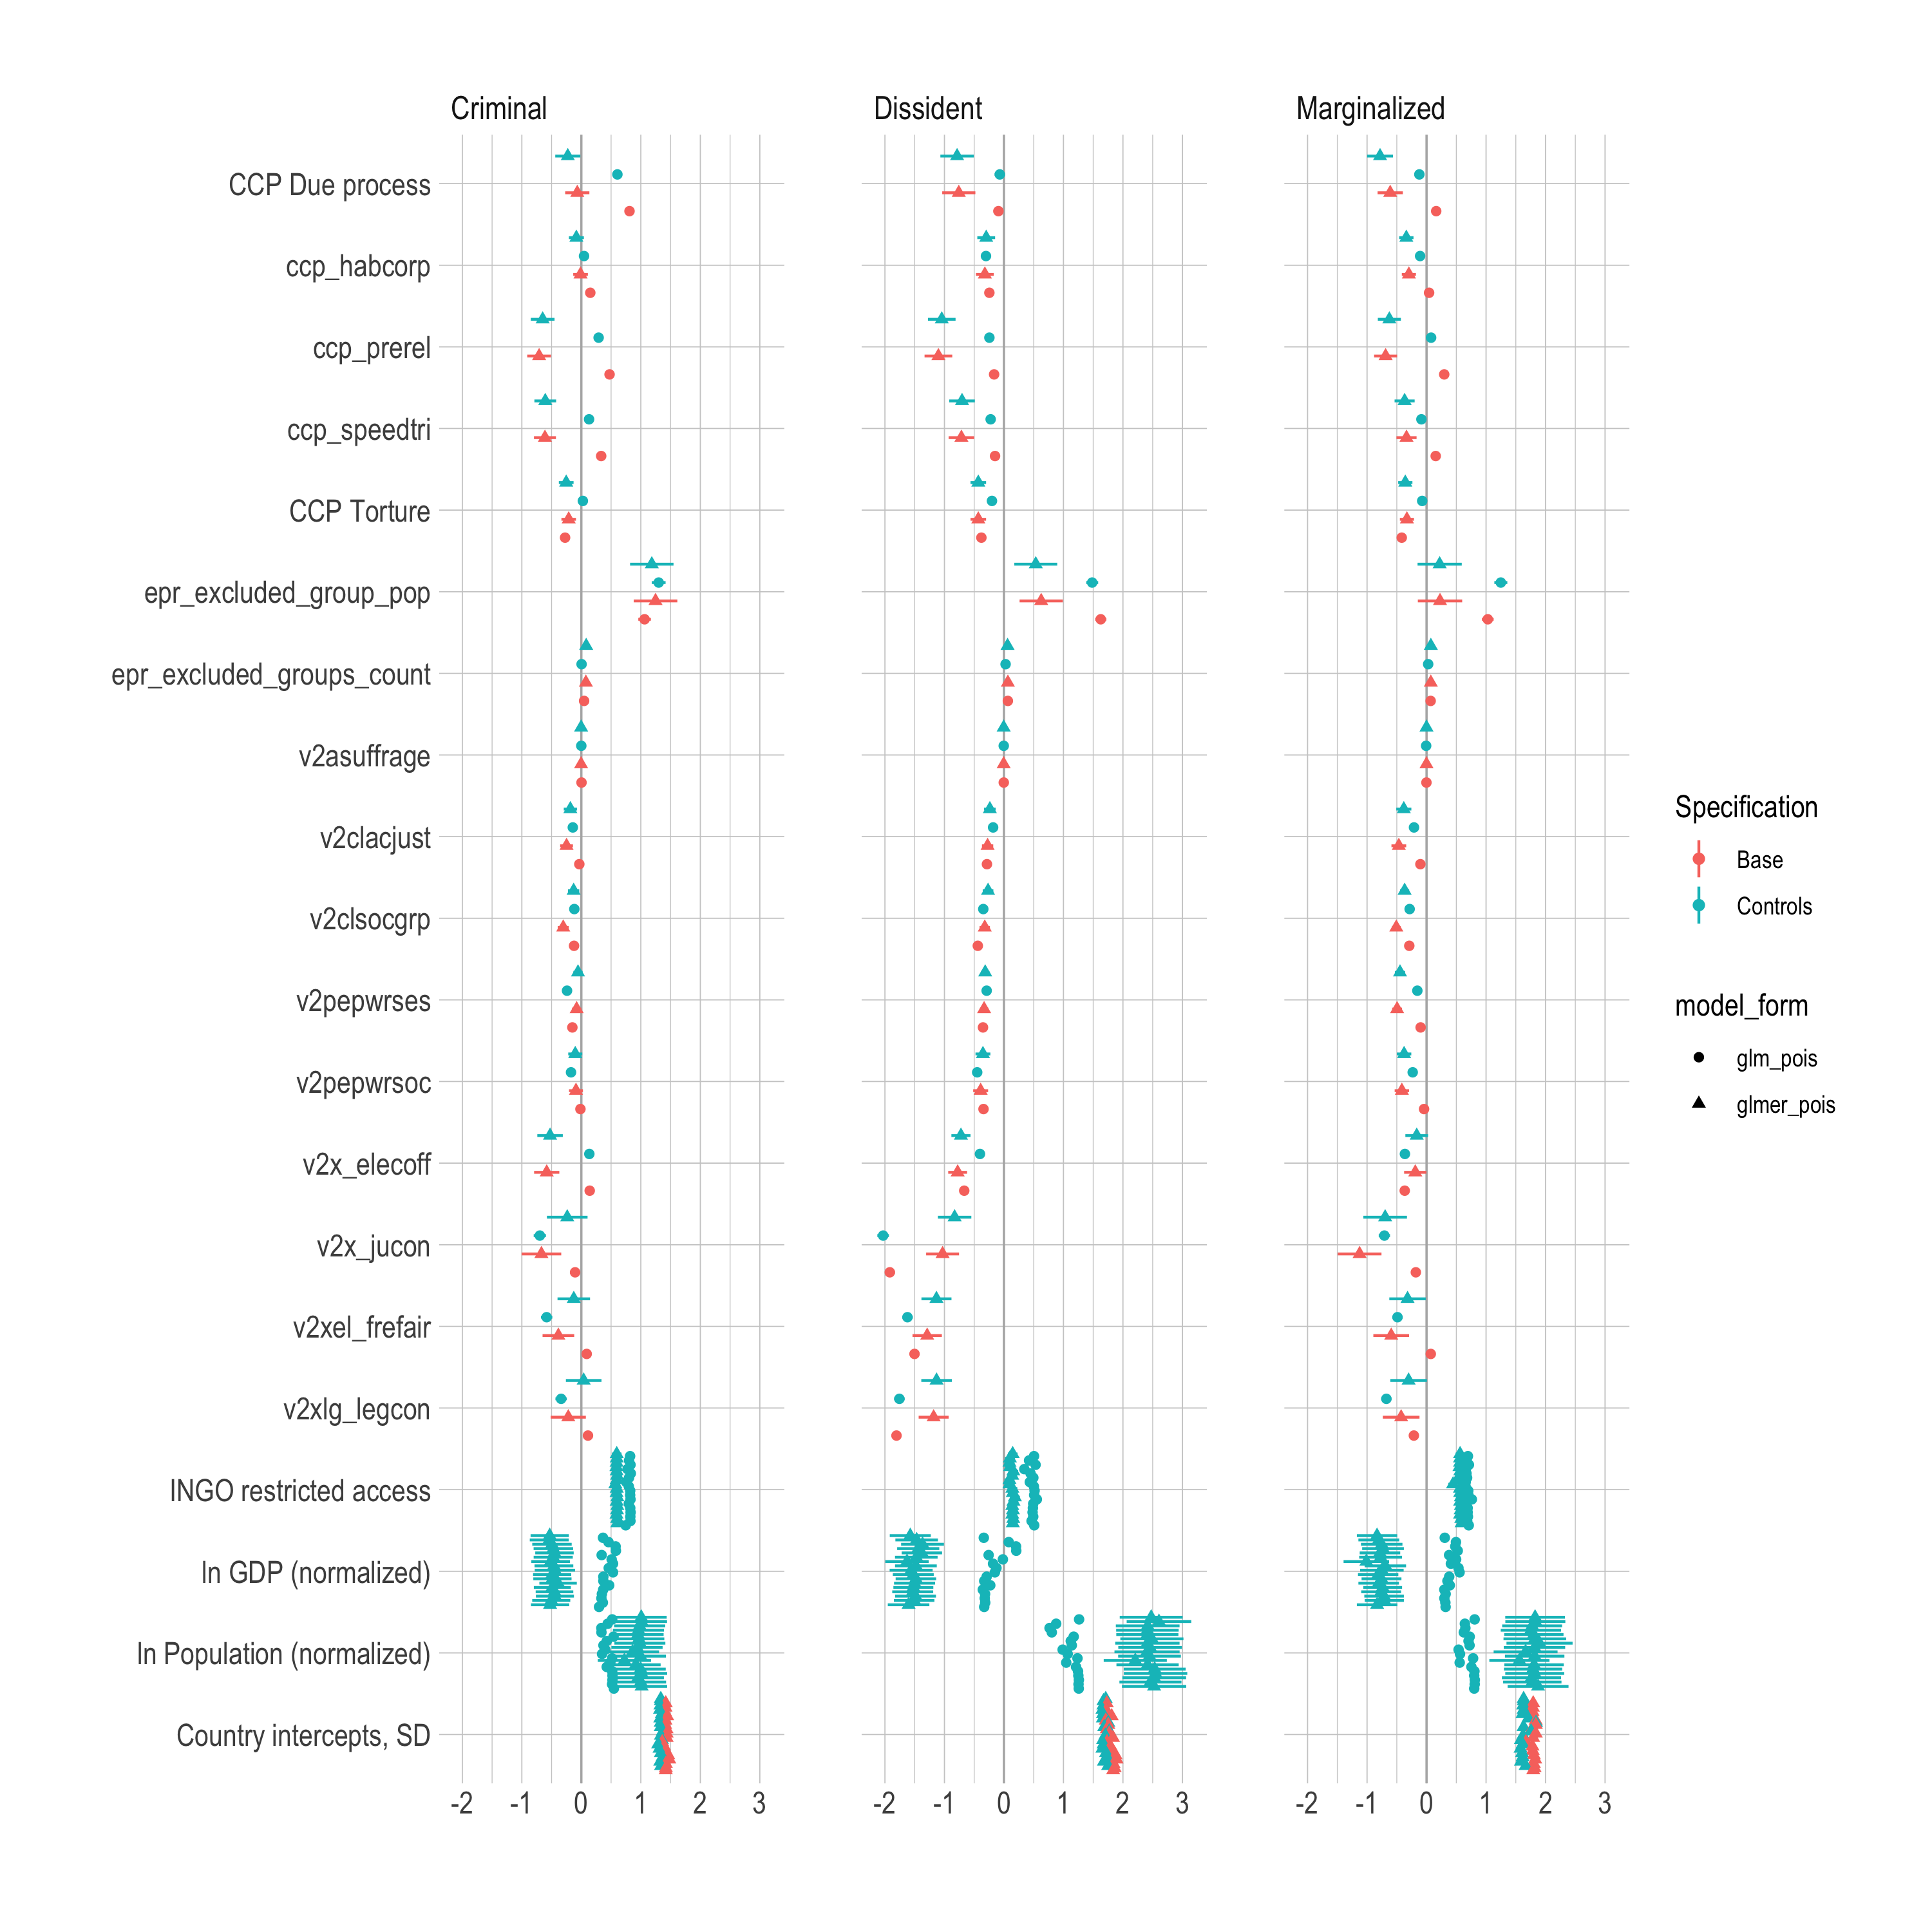
\includegraphics[width=.9\textwidth]{../output/figures/model-coefs-all-model-forms.png}
\end{figure}

\begin{figure}
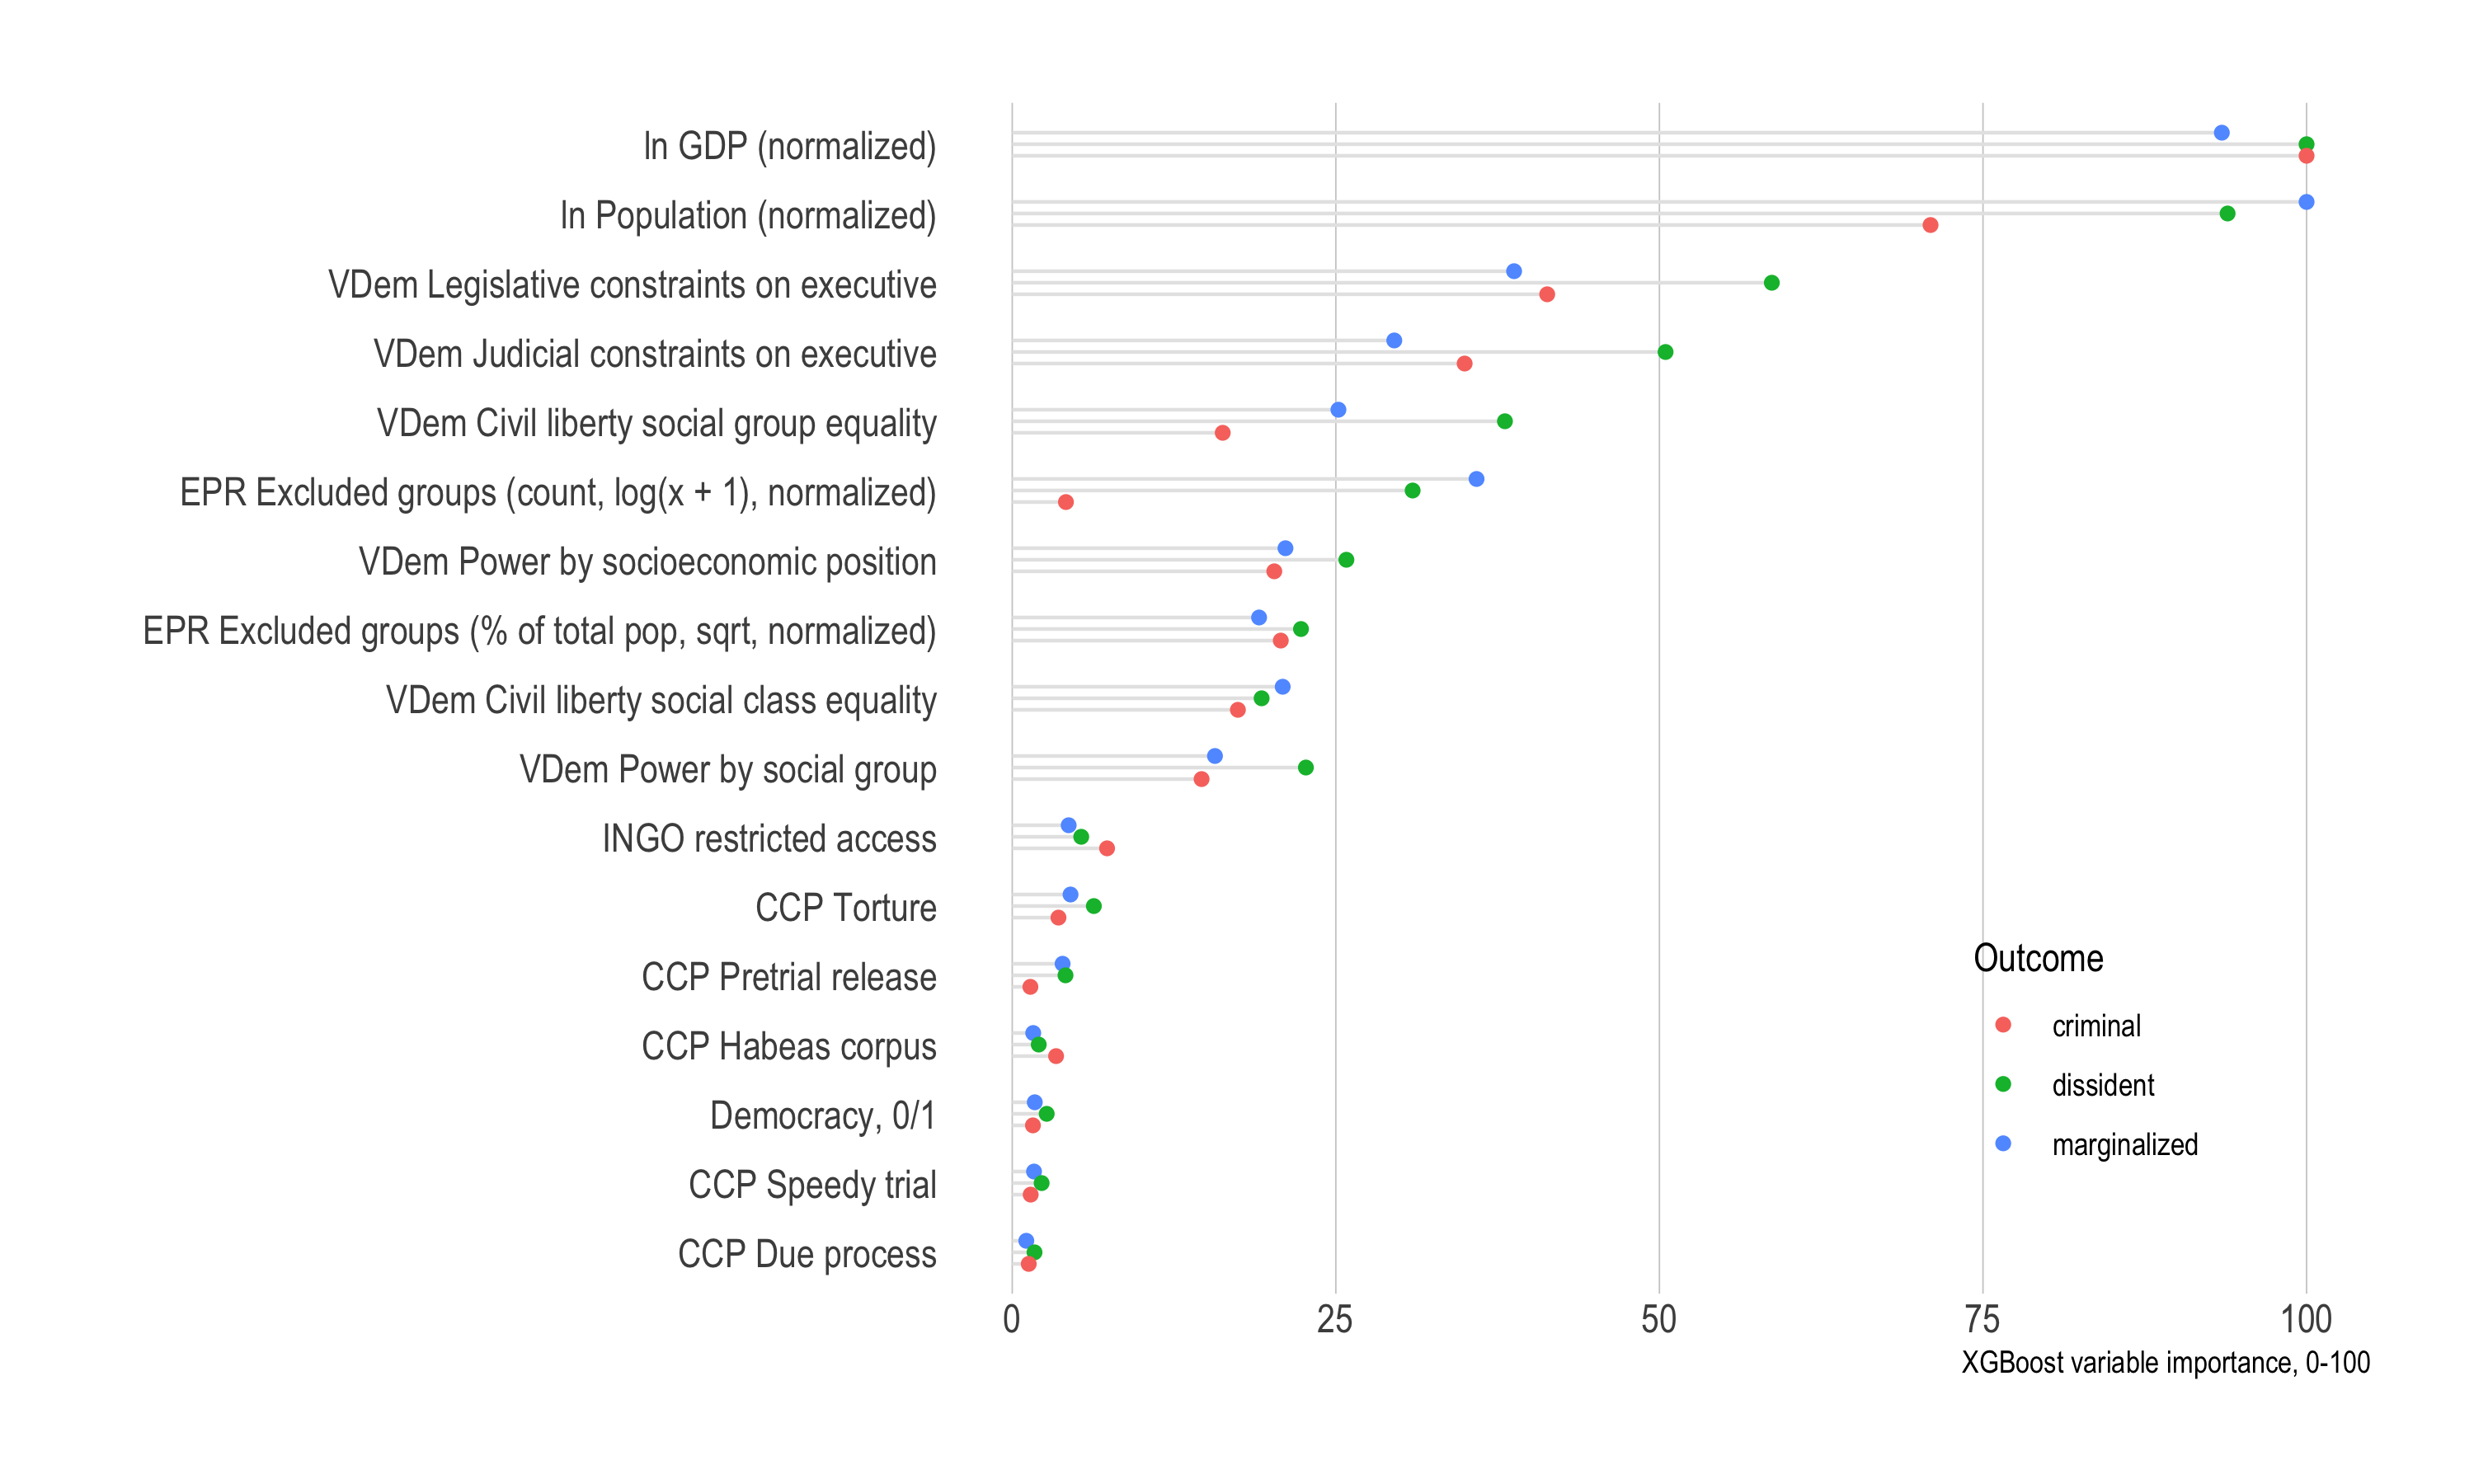
\includegraphics[width=.9\textwidth]{../output/figures/xgboost-variable-importance-v1.png}
\end{figure}

\begin{figure}
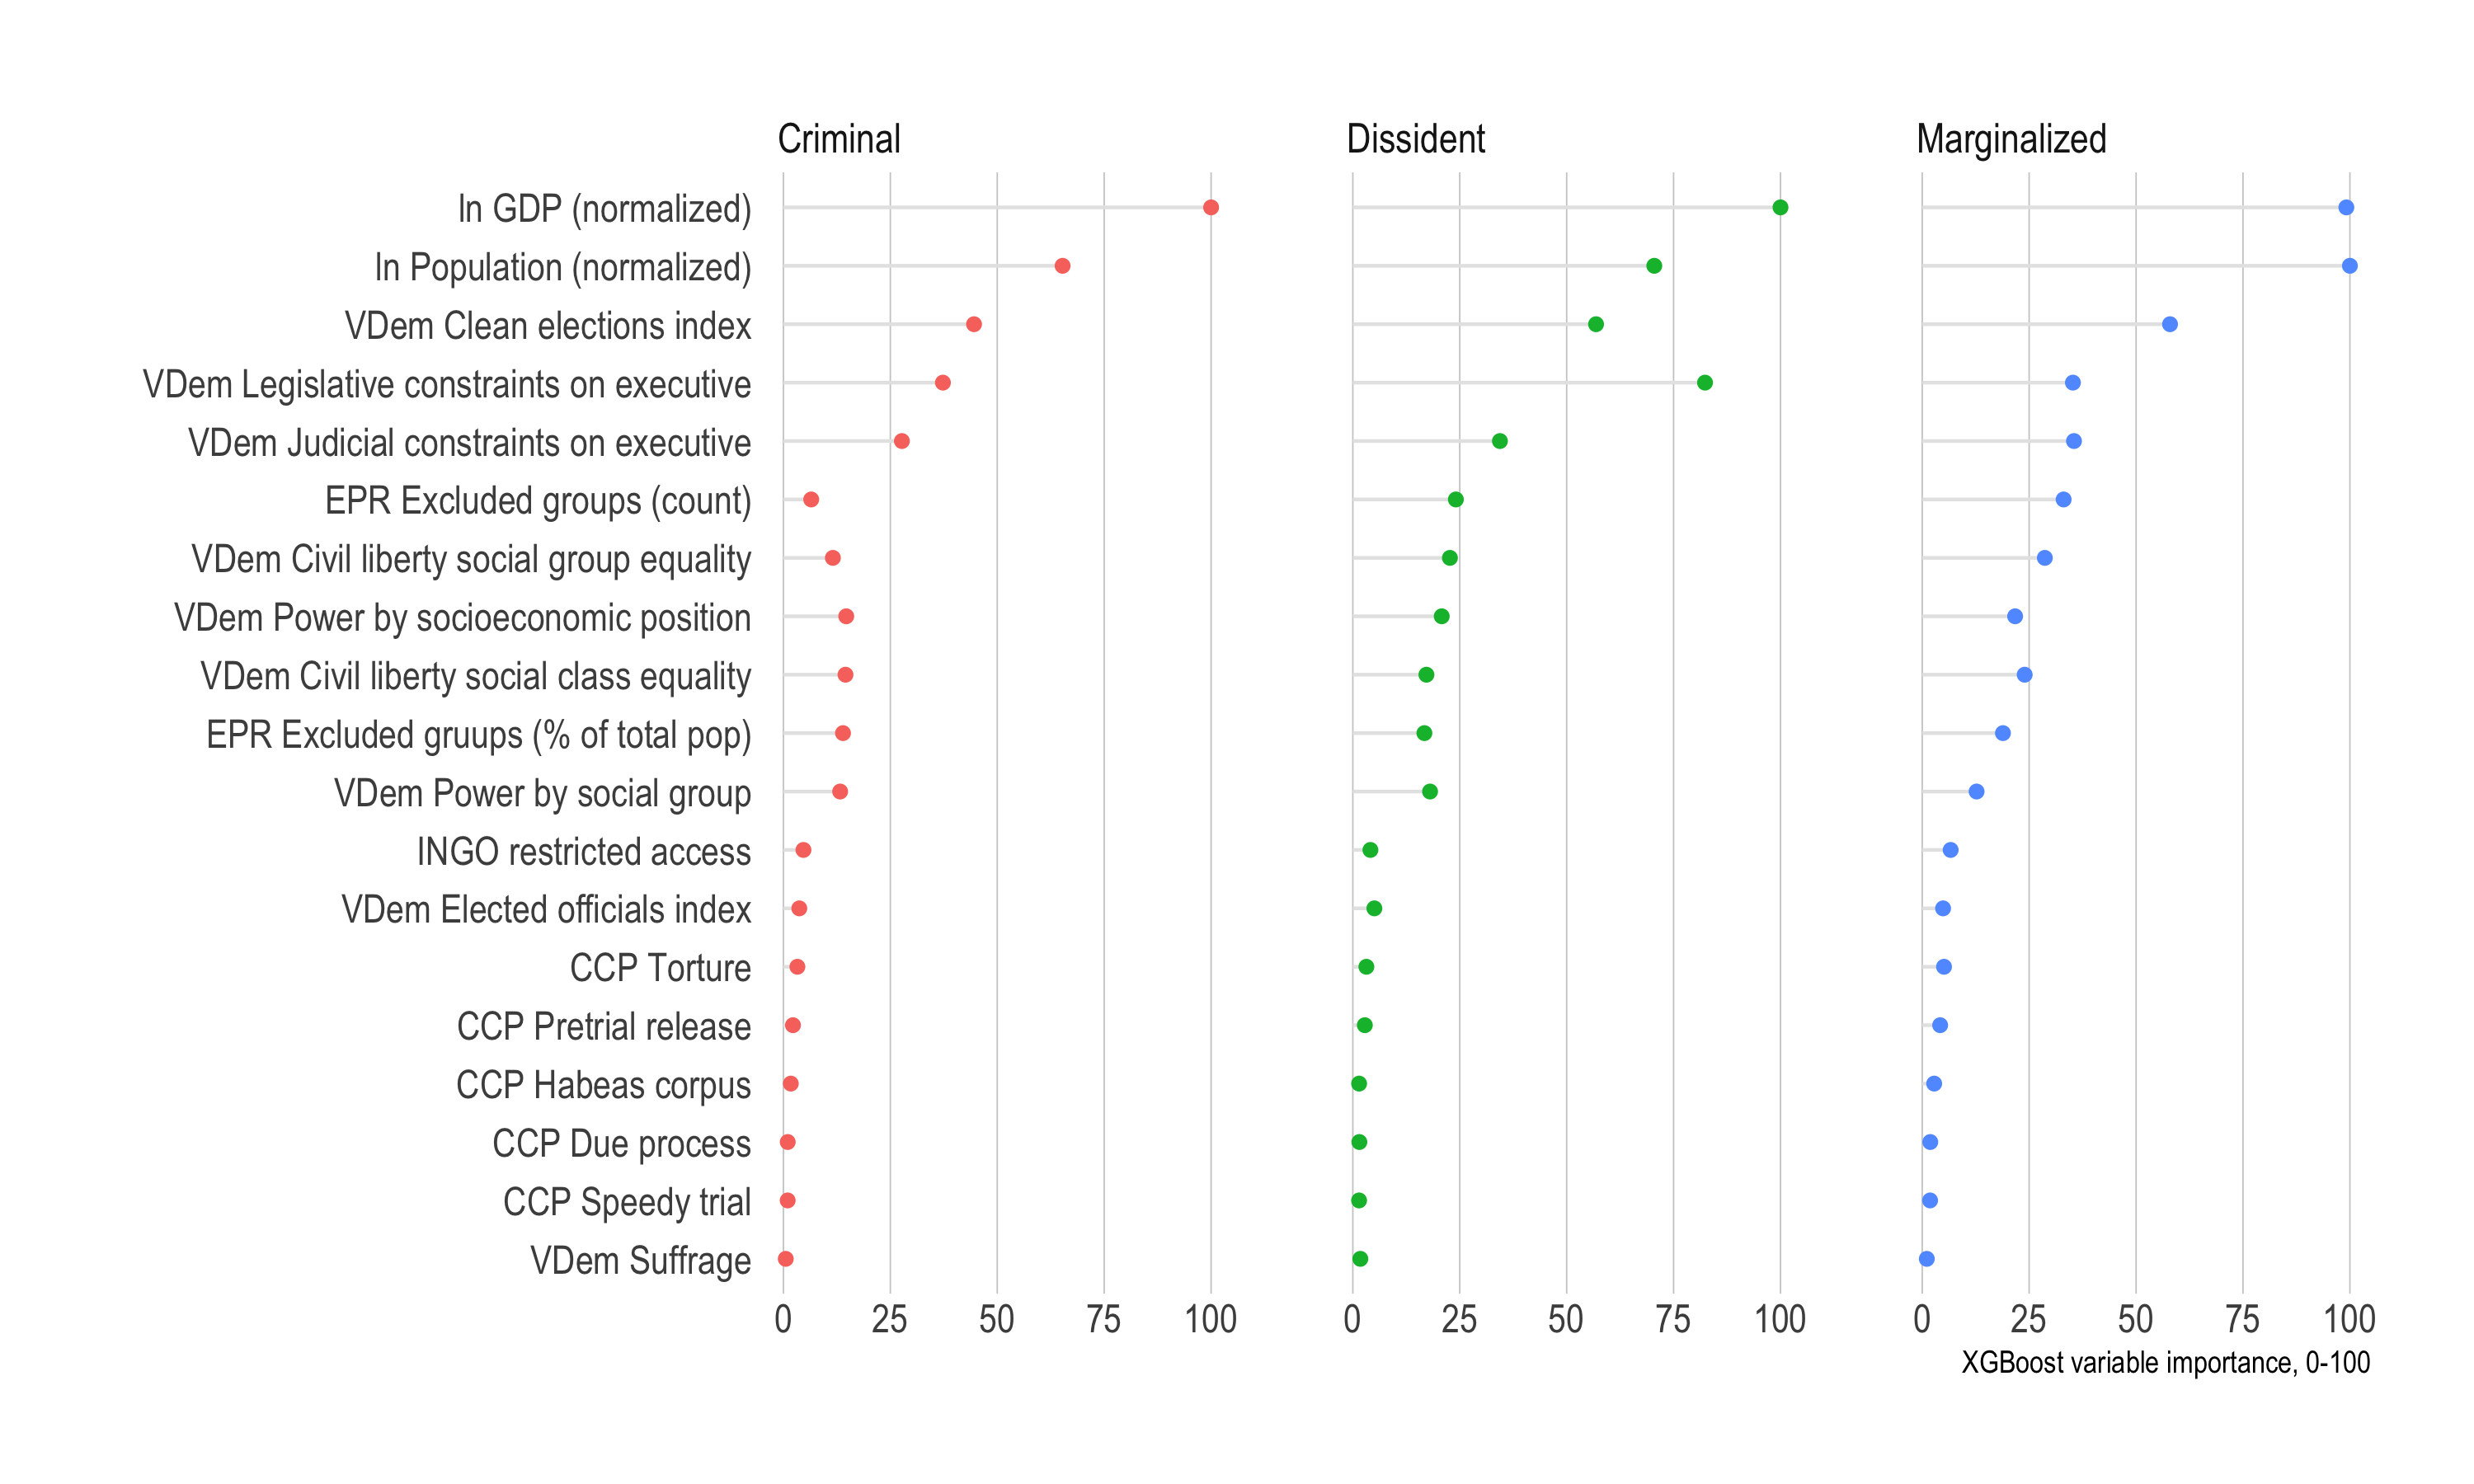
\includegraphics[width=.9\textwidth]{../output/figures/xgboost-variable-importance-v2.png}
\end{figure}

\begin{figure}
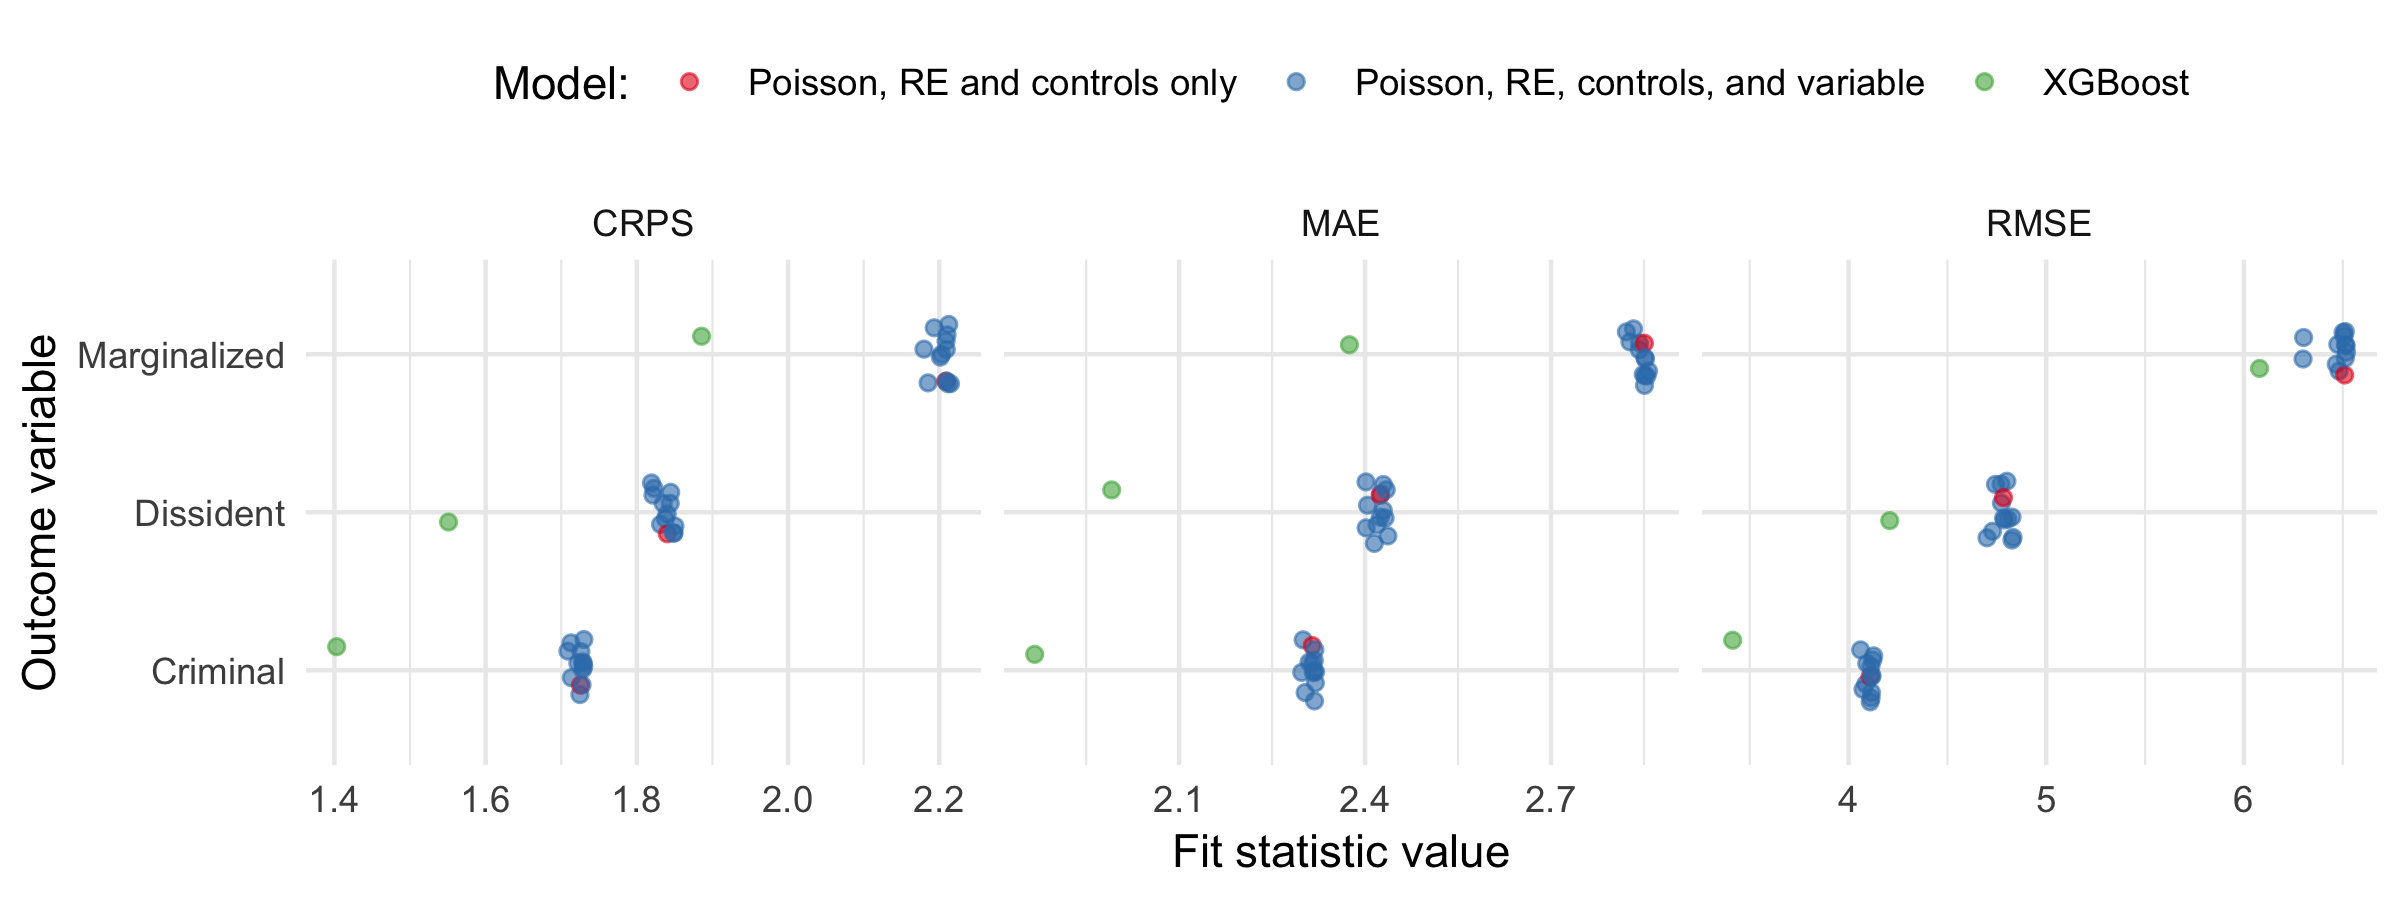
\includegraphics[width=.9\textwidth]{../output/figures/oos-fit-all.png}
\end{figure}


% Tables

% Table created by stargazer v.5.2.2 by Marek Hlavac, Harvard University. E-mail: hlavac at fas.harvard.edu
% Date and time: Sun, Jan 27, 2019 - 21:11:12
% Requires LaTeX packages: rotating 
\begin{sidewaystable}[!htbp] \centering 
  \caption{} 
  \label{} 
\tiny 
\begin{tabular}{@{\extracolsep{5pt}}lccccccccc} 
\\[-1.8ex]\hline 
\hline \\[-1.8ex] 
 & \multicolumn{9}{c}{\textit{Dependent variable:}} \\ 
\cline{2-10} 
\\[-1.8ex] & \multicolumn{9}{c}{itt\_alleg\_vtcriminal} \\ 
\\[-1.8ex] & (1) & (2) & (3) & (4) & (5) & (6) & (7) & (8) & (9)\\ 
\hline \\[-1.8ex] 
 ccp\_torture &  & $-$0.254$^{***}$ &  &  &  &  &  &  &  \\ 
  &  & (0.063) &  &  &  &  &  &  &  \\ 
  ccp\_prerel &  &  & $-$0.650$^{***}$ &  &  &  &  &  &  \\ 
  &  &  & (0.102) &  &  &  &  &  &  \\ 
  ccp\_habcorp &  &  &  & $-$0.083 &  &  &  &  &  \\ 
  &  &  &  & (0.064) &  &  &  &  &  \\ 
  ccp\_dueproc &  &  &  &  & $-$0.227$^{**}$ &  &  &  &  \\ 
  &  &  &  &  & (0.108) &  &  &  &  \\ 
  ccp\_speedtri &  &  &  &  &  & $-$0.606$^{***}$ &  &  &  \\ 
  &  &  &  &  &  & (0.093) &  &  &  \\ 
  v2x\_elecoff &  &  &  &  &  &  & $-$0.526$^{***}$ &  &  \\ 
  &  &  &  &  &  &  & (0.109) &  &  \\ 
  v2xel\_frefair &  &  &  &  &  &  &  & $-$0.127 &  \\ 
  &  &  &  &  &  &  &  & (0.139) &  \\ 
  v2asuffrage &  &  &  &  &  &  &  &  & $-$0.003$^{***}$ \\ 
  &  &  &  &  &  &  &  &  & (0.001) \\ 
  norm\_ln\_NY.GDP.MKTP.KD & $-$0.531$^{***}$ & $-$0.487$^{***}$ & $-$0.444$^{***}$ & $-$0.506$^{***}$ & $-$0.525$^{***}$ & $-$0.451$^{***}$ & $-$0.451$^{***}$ & $-$0.494$^{***}$ & $-$0.491$^{***}$ \\ 
  & (0.164) & (0.159) & (0.163) & (0.163) & (0.164) & (0.161) & (0.165) & (0.169) & (0.164) \\ 
  norm\_ln\_pop & 1.007$^{***}$ & 0.997$^{***}$ & 0.953$^{***}$ & 1.000$^{***}$ & 1.013$^{***}$ & 1.014$^{***}$ & 0.951$^{***}$ & 0.981$^{***}$ & 0.995$^{***}$ \\ 
  & (0.218) & (0.215) & (0.222) & (0.217) & (0.219) & (0.218) & (0.221) & (0.219) & (0.218) \\ 
  itt\_RstrctAccess & 0.595$^{***}$ & 0.605$^{***}$ & 0.592$^{***}$ & 0.601$^{***}$ & 0.604$^{***}$ & 0.599$^{***}$ & 0.594$^{***}$ & 0.593$^{***}$ & 0.592$^{***}$ \\ 
  & (0.041) & (0.041) & (0.041) & (0.041) & (0.041) & (0.041) & (0.041) & (0.041) & (0.041) \\ 
  Constant & 0.135 & 0.276$^{**}$ & 0.240$^{*}$ & 0.183 & 0.152 & 0.264$^{**}$ & 0.564$^{***}$ & 0.203 & 0.437$^{***}$ \\ 
  & (0.132) & (0.135) & (0.136) & (0.137) & (0.133) & (0.134) & (0.160) & (0.151) & (0.157) \\ 
 \hline \\[-1.8ex] 
Observations & 1,654 & 1,654 & 1,654 & 1,654 & 1,654 & 1,654 & 1,654 & 1,654 & 1,654 \\ 
Log Likelihood & $-$3,834.972 & $-$3,826.947 & $-$3,814.044 & $-$3,834.140 & $-$3,832.781 & $-$3,812.073 & $-$3,823.631 & $-$3,834.563 & $-$3,828.828 \\ 
Akaike Inf. Crit. & 7,679.944 & 7,665.893 & 7,640.088 & 7,680.280 & 7,677.562 & 7,636.145 & 7,659.262 & 7,681.127 & 7,669.655 \\ 
Bayesian Inf. Crit. & 7,706.999 & 7,698.359 & 7,672.554 & 7,712.746 & 7,710.028 & 7,668.611 & 7,691.728 & 7,713.592 & 7,702.121 \\ 
\hline 
\hline \\[-1.8ex] 
\textit{Note:}  & \multicolumn{9}{r}{$^{*}$p$<$0.1; $^{**}$p$<$0.05; $^{***}$p$<$0.01} \\ 
\end{tabular} 
\end{sidewaystable} 


% Table created by stargazer v.5.2.2 by Marek Hlavac, Harvard University. E-mail: hlavac at fas.harvard.edu
% Date and time: Sat, Feb 02, 2019 - 20:56:40
% Requires LaTeX packages: rotating 
\begin{sidewaystable}[!htbp] \centering 
  \caption{} 
  \label{} 
\tiny 
\begin{tabular}{@{\extracolsep{5pt}}lcccccccc} 
\\[-1.8ex]\hline 
\hline \\[-1.8ex] 
 & \multicolumn{8}{c}{\textit{Dependent variable:}} \\ 
\cline{2-9} 
\\[-1.8ex] & \multicolumn{8}{c}{Criminal} \\ 
\\[-1.8ex] & (1) & (2) & (3) & (4) & (5) & (6) & (7) & (8)\\ 
\hline \\[-1.8ex] 
 VDem Legislative constraints on executive & 0.047 &  &  &  &  &  &  &  \\ 
  & (0.153) &  &  &  &  &  &  &  \\ 
  VDem Civil liberty social class equality &  & $-$0.186$^{***}$ &  &  &  &  &  &  \\ 
  &  & (0.057) &  &  &  &  &  &  \\ 
  VDem Civil liberty social group equality &  &  & $-$0.127$^{***}$ &  &  &  &  &  \\ 
  &  &  & (0.048) &  &  &  &  &  \\ 
  VDem Power by socioeconomic position &  &  &  & $-$0.056 &  &  &  &  \\ 
  &  &  &  & (0.040) &  &  &  &  \\ 
  VDem Power by social group &  &  &  &  & $-$0.097 &  &  &  \\ 
  &  &  &  &  & (0.061) &  &  &  \\ 
  norm\_sqrt\_epr\_excluded\_group\_pop &  &  &  &  &  & 0.236$^{***}$ &  &  \\ 
  &  &  &  &  &  & (0.039) &  &  \\ 
  EPR Excluded groups (count, log(x + 1), normalized) &  &  &  &  &  &  & 0.343$^{***}$ &  \\ 
  &  &  &  &  &  &  & (0.066) &  \\ 
  dd\_democracy &  &  &  &  &  &  &  & $-$0.281$^{***}$ \\ 
  &  &  &  &  &  &  &  & (0.074) \\ 
  ln GDP (normalized) & $-$0.457$^{***}$ & $-$0.374$^{**}$ & $-$0.391$^{***}$ & $-$0.436$^{***}$ & $-$0.402$^{***}$ & $-$0.325$^{**}$ & $-$0.363$^{***}$ & $-$0.366$^{***}$ \\ 
  & (0.142) & (0.147) & (0.141) & (0.141) & (0.143) & (0.136) & (0.136) & (0.140) \\ 
  ln Population (normalized) & 0.641$^{***}$ & 0.542$^{***}$ & 0.595$^{***}$ & 0.623$^{***}$ & 0.615$^{***}$ & 0.564$^{***}$ & 0.464$^{***}$ & 0.611$^{***}$ \\ 
  & (0.140) & (0.146) & (0.141) & (0.140) & (0.140) & (0.136) & (0.141) & (0.139) \\ 
  ACD Internal conflict & 0.044 & 0.049 & 0.031 & 0.043 & 0.031 & 0.033 & 0.031 & 0.036 \\ 
  & (0.050) & (0.050) & (0.050) & (0.050) & (0.051) & (0.050) & (0.050) & (0.050) \\ 
  INGO restricted access & 0.600$^{***}$ & 0.600$^{***}$ & 0.575$^{***}$ & 0.599$^{***}$ & 0.603$^{***}$ & 0.599$^{***}$ & 0.602$^{***}$ & 0.580$^{***}$ \\ 
  & (0.041) & (0.041) & (0.043) & (0.041) & (0.041) & (0.041) & (0.041) & (0.042) \\ 
  Global intercept & 0.344$^{**}$ & 0.518$^{***}$ & 0.485$^{***}$ & 0.399$^{***}$ & 0.440$^{***}$ & 0.375$^{***}$ & 0.373$^{***}$ & 0.524$^{***}$ \\ 
  & (0.144) & (0.125) & (0.121) & (0.115) & (0.121) & (0.109) & (0.110) & (0.119) \\ 
 \hline \\[-1.8ex] 
Observations & 1,654 & 1,654 & 1,654 & 1,654 & 1,654 & 1,654 & 1,654 & 1,654 \\ 
Log Likelihood & $-$3,834.565 & $-$3,829.193 & $-$3,831.180 & $-$3,833.618 & $-$3,833.359 & $-$3,814.756 & $-$3,821.128 & $-$3,827.512 \\ 
Akaike Inf. Crit. & 7,683.129 & 7,672.385 & 7,676.361 & 7,681.236 & 7,680.718 & 7,643.512 & 7,656.257 & 7,669.023 \\ 
Bayesian Inf. Crit. & 7,721.006 & 7,710.262 & 7,714.238 & 7,719.113 & 7,718.594 & 7,681.389 & 7,694.134 & 7,706.900 \\ 
\hline 
\hline \\[-1.8ex] 
\textit{Note:}  & \multicolumn{8}{r}{$^{*}$p$<$0.1; $^{**}$p$<$0.05; $^{***}$p$<$0.01} \\ 
\end{tabular} 
\end{sidewaystable} 



% Table created by stargazer v.5.2.2 by Marek Hlavac, Harvard University. E-mail: hlavac at fas.harvard.edu
% Date and time: Sat, Feb 02, 2019 - 20:56:44
% Requires LaTeX packages: rotating 
\begin{sidewaystable}[!htbp] \centering 
  \caption{} 
  \label{} 
\tiny 
\begin{tabular}{@{\extracolsep{5pt}}lccccccc} 
\\[-1.8ex]\hline 
\hline \\[-1.8ex] 
 & \multicolumn{7}{c}{\textit{Dependent variable:}} \\ 
\cline{2-8} 
\\[-1.8ex] & \multicolumn{7}{c}{Dissident} \\ 
\\[-1.8ex] & (1) & (2) & (3) & (4) & (5) & (6) & (7)\\ 
\hline \\[-1.8ex] 
 CCP Torture &  & $-$0.482$^{***}$ &  &  &  &  &  \\ 
  &  & (0.068) &  &  &  &  &  \\ 
  CCP Pretrial release &  &  & $-$1.052$^{***}$ &  &  &  &  \\ 
  &  &  & (0.119) &  &  &  &  \\ 
  CCP Habeas corpus &  &  &  & $-$0.301$^{***}$ &  &  &  \\ 
  &  &  &  & (0.077) &  &  &  \\ 
  CCP Due process &  &  &  &  & $-$0.795$^{***}$ &  &  \\ 
  &  &  &  &  & (0.144) &  &  \\ 
  CCP Speedy trial &  &  &  &  &  & $-$0.711$^{***}$ &  \\ 
  &  &  &  &  &  & (0.110) &  \\ 
  VDem Judicial constraints on executive &  &  &  &  &  &  & $-$0.940$^{***}$ \\ 
  &  &  &  &  &  &  & (0.145) \\ 
  ln GDP (normalized) & $-$1.296$^{***}$ & $-$1.242$^{***}$ & $-$1.215$^{***}$ & $-$1.239$^{***}$ & $-$1.321$^{***}$ & $-$1.257$^{***}$ & $-$1.163$^{***}$ \\ 
  & (0.150) & (0.146) & (0.149) & (0.148) & (0.152) & (0.150) & (0.155) \\ 
  ln Population (normalized) & 1.519$^{***}$ & 1.549$^{***}$ & 1.548$^{***}$ & 1.510$^{***}$ & 1.551$^{***}$ & 1.562$^{***}$ & 1.464$^{***}$ \\ 
  & (0.173) & (0.170) & (0.175) & (0.171) & (0.177) & (0.175) & (0.172) \\ 
  ACD Internal conflict & 0.403$^{***}$ & 0.434$^{***}$ & 0.407$^{***}$ & 0.405$^{***}$ & 0.405$^{***}$ & 0.407$^{***}$ & 0.426$^{***}$ \\ 
  & (0.053) & (0.053) & (0.053) & (0.053) & (0.053) & (0.054) & (0.053) \\ 
  INGO restricted access & 0.161$^{***}$ & 0.156$^{***}$ & 0.155$^{***}$ & 0.170$^{***}$ & 0.163$^{***}$ & 0.164$^{***}$ & 0.116$^{***}$ \\ 
  & (0.042) & (0.042) & (0.041) & (0.042) & (0.042) & (0.042) & (0.043) \\ 
  Global intercept & $-$0.053 & 0.227 & 0.118 & 0.139 & 0.015 & 0.123 & 0.471$^{***}$ \\ 
  & (0.147) & (0.147) & (0.149) & (0.152) & (0.151) & (0.150) & (0.164) \\ 
 \hline \\[-1.8ex] 
Observations & 1,654 & 1,654 & 1,654 & 1,654 & 1,654 & 1,654 & 1,654 \\ 
Log Likelihood & $-$3,826.920 & $-$3,801.365 & $-$3,784.456 & $-$3,819.157 & $-$3,810.642 & $-$3,804.919 & $-$3,806.070 \\ 
Akaike Inf. Crit. & 7,665.840 & 7,616.730 & 7,582.912 & 7,652.315 & 7,635.284 & 7,623.838 & 7,626.140 \\ 
Bayesian Inf. Crit. & 7,698.306 & 7,654.607 & 7,620.788 & 7,690.192 & 7,673.161 & 7,661.715 & 7,664.017 \\ 
\hline 
\hline \\[-1.8ex] 
\textit{Note:}  & \multicolumn{7}{r}{$^{*}$p$<$0.1; $^{**}$p$<$0.05; $^{***}$p$<$0.01} \\ 
\end{tabular} 
\end{sidewaystable} 


% Table created by stargazer v.5.2.2 by Marek Hlavac, Harvard University. E-mail: hlavac at fas.harvard.edu
% Date and time: Sun, Jan 27, 2019 - 21:11:27
% Requires LaTeX packages: rotating 
\begin{sidewaystable}[!htbp] \centering 
  \caption{} 
  \label{} 
\tiny 
\begin{tabular}{@{\extracolsep{5pt}}lcccccccc} 
\\[-1.8ex]\hline 
\hline \\[-1.8ex] 
 & \multicolumn{8}{c}{\textit{Dependent variable:}} \\ 
\cline{2-9} 
\\[-1.8ex] & \multicolumn{8}{c}{itt\_alleg\_vtdissident} \\ 
\\[-1.8ex] & (1) & (2) & (3) & (4) & (5) & (6) & (7) & (8)\\ 
\hline \\[-1.8ex] 
 v2x\_jucon & $-$0.829$^{***}$ &  &  &  &  &  &  &  \\ 
  & (0.143) &  &  &  &  &  &  &  \\ 
  v2xlg\_legcon &  & $-$1.132$^{***}$ &  &  &  &  &  &  \\ 
  &  & (0.131) &  &  &  &  &  &  \\ 
  v2clacjust &  &  & $-$0.237$^{***}$ &  &  &  &  &  \\ 
  &  &  & (0.050) &  &  &  &  &  \\ 
  v2clsocgrp &  &  &  & $-$0.267$^{***}$ &  &  &  &  \\ 
  &  &  &  & (0.046) &  &  &  &  \\ 
  v2pepwrses &  &  &  &  & $-$0.315$^{***}$ &  &  &  \\ 
  &  &  &  &  & (0.036) &  &  &  \\ 
  v2pepwrsoc &  &  &  &  &  & $-$0.353$^{***}$ &  &  \\ 
  &  &  &  &  &  & (0.064) &  &  \\ 
  epr\_excluded\_groups\_count &  &  &  &  &  &  & 0.061$^{***}$ &  \\ 
  &  &  &  &  &  &  & (0.014) &  \\ 
  epr\_excluded\_group\_pop &  &  &  &  &  &  &  & 0.535$^{***}$ \\ 
  &  &  &  &  &  &  &  & (0.184) \\ 
  norm\_ln\_NY.GDP.MKTP.KD & $-$1.441$^{***}$ & $-$1.467$^{***}$ & $-$1.560$^{***}$ & $-$1.480$^{***}$ & $-$1.629$^{***}$ & $-$1.473$^{***}$ & $-$1.480$^{***}$ & $-$1.502$^{***}$ \\ 
  & (0.181) & (0.182) & (0.184) & (0.179) & (0.186) & (0.183) & (0.174) & (0.176) \\ 
  norm\_ln\_pop & 2.411$^{***}$ & 2.605$^{***}$ & 2.405$^{***}$ & 2.456$^{***}$ & 2.411$^{***}$ & 2.486$^{***}$ & 2.207$^{***}$ & 2.414$^{***}$ \\ 
  & (0.268) & (0.277) & (0.279) & (0.272) & (0.276) & (0.271) & (0.271) & (0.267) \\ 
  itt\_RstrctAccess & 0.104$^{**}$ & 0.100$^{**}$ & 0.142$^{***}$ & 0.091$^{**}$ & 0.093$^{**}$ & 0.139$^{***}$ & 0.184$^{***}$ & 0.159$^{***}$ \\ 
  & (0.043) & (0.043) & (0.042) & (0.043) & (0.043) & (0.042) & (0.042) & (0.042) \\ 
  Constant & $-$0.048 & 0.046 & $-$0.309$^{*}$ & $-$0.297$^{*}$ & $-$0.332$^{*}$ & $-$0.306$^{*}$ & $-$0.574$^{***}$ & $-$0.575$^{***}$ \\ 
  & (0.185) & (0.182) & (0.182) & (0.175) & (0.177) & (0.172) & (0.169) & (0.171) \\ 
 \hline \\[-1.8ex] 
Observations & 1,654 & 1,654 & 1,654 & 1,654 & 1,654 & 1,654 & 1,654 & 1,654 \\ 
Log Likelihood & $-$3,838.513 & $-$3,817.959 & $-$3,843.958 & $-$3,837.750 & $-$3,816.799 & $-$3,839.851 & $-$3,845.627 & $-$3,850.900 \\ 
Akaike Inf. Crit. & 7,689.026 & 7,647.919 & 7,699.916 & 7,687.500 & 7,645.597 & 7,691.702 & 7,703.254 & 7,713.801 \\ 
Bayesian Inf. Crit. & 7,721.491 & 7,680.385 & 7,732.382 & 7,719.966 & 7,678.063 & 7,724.168 & 7,735.720 & 7,746.266 \\ 
\hline 
\hline \\[-1.8ex] 
\textit{Note:}  & \multicolumn{8}{r}{$^{*}$p$<$0.1; $^{**}$p$<$0.05; $^{***}$p$<$0.01} \\ 
\end{tabular} 
\end{sidewaystable} 



% Table created by stargazer v.5.2.2 by Marek Hlavac, Harvard University. E-mail: hlavac at fas.harvard.edu
% Date and time: Sat, Feb 02, 2019 - 20:56:52
% Requires LaTeX packages: rotating 
\begin{sidewaystable}[!htbp] \centering 
  \caption{} 
  \label{} 
\tiny 
\begin{tabular}{@{\extracolsep{5pt}}lccccccc} 
\\[-1.8ex]\hline 
\hline \\[-1.8ex] 
 & \multicolumn{7}{c}{\textit{Dependent variable:}} \\ 
\cline{2-8} 
\\[-1.8ex] & \multicolumn{7}{c}{Marginalized} \\ 
\\[-1.8ex] & (1) & (2) & (3) & (4) & (5) & (6) & (7)\\ 
\hline \\[-1.8ex] 
 CCP Torture &  & $-$0.358$^{***}$ &  &  &  &  &  \\ 
  &  & (0.061) &  &  &  &  &  \\ 
  CCP Pretrial release &  &  & $-$0.610$^{***}$ &  &  &  &  \\ 
  &  &  & (0.098) &  &  &  &  \\ 
  CCP Habeas corpus &  &  &  & $-$0.335$^{***}$ &  &  &  \\ 
  &  &  &  & (0.061) &  &  &  \\ 
  CCP Due process &  &  &  &  & $-$0.795$^{***}$ &  &  \\ 
  &  &  &  &  & (0.111) &  &  \\ 
  CCP Speedy trial &  &  &  &  &  & $-$0.367$^{***}$ &  \\ 
  &  &  &  &  &  & (0.086) &  \\ 
  VDem Judicial constraints on executive &  &  &  &  &  &  & $-$0.692$^{***}$ \\ 
  &  &  &  &  &  &  & (0.188) \\ 
  ln GDP (normalized) & $-$0.695$^{***}$ & $-$0.612$^{***}$ & $-$0.592$^{***}$ & $-$0.590$^{***}$ & $-$0.695$^{***}$ & $-$0.634$^{***}$ & $-$0.610$^{***}$ \\ 
  & (0.149) & (0.143) & (0.146) & (0.144) & (0.149) & (0.147) & (0.154) \\ 
  ln Population (normalized) & 1.132$^{***}$ & 1.105$^{***}$ & 1.092$^{***}$ & 1.100$^{***}$ & 1.164$^{***}$ & 1.126$^{***}$ & 1.086$^{***}$ \\ 
  & (0.164) & (0.160) & (0.162) & (0.161) & (0.168) & (0.162) & (0.166) \\ 
  ACD Internal conflict & 0.313$^{***}$ & 0.312$^{***}$ & 0.303$^{***}$ & 0.308$^{***}$ & 0.321$^{***}$ & 0.313$^{***}$ & 0.310$^{***}$ \\ 
  & (0.055) & (0.055) & (0.055) & (0.055) & (0.055) & (0.055) & (0.055) \\ 
  INGO restricted access & 0.585$^{***}$ & 0.599$^{***}$ & 0.584$^{***}$ & 0.604$^{***}$ & 0.612$^{***}$ & 0.594$^{***}$ & 0.575$^{***}$ \\ 
  & (0.038) & (0.038) & (0.038) & (0.039) & (0.039) & (0.038) & (0.039) \\ 
  Global intercept & 0.092 & 0.310$^{**}$ & 0.204 & 0.307$^{**}$ & 0.157 & 0.192 & 0.477$^{***}$ \\ 
  & (0.139) & (0.140) & (0.139) & (0.141) & (0.143) & (0.139) & (0.174) \\ 
 \hline \\[-1.8ex] 
Observations & 1,654 & 1,654 & 1,654 & 1,654 & 1,654 & 1,654 & 1,654 \\ 
Log Likelihood & $-$4,187.693 & $-$4,170.539 & $-$4,167.731 & $-$4,172.666 & $-$4,161.722 & $-$4,178.291 & $-$4,180.898 \\ 
Akaike Inf. Crit. & 8,387.386 & 8,355.078 & 8,349.461 & 8,359.332 & 8,337.445 & 8,370.581 & 8,375.796 \\ 
Bayesian Inf. Crit. & 8,419.852 & 8,392.955 & 8,387.338 & 8,397.208 & 8,375.321 & 8,408.458 & 8,413.673 \\ 
\hline 
\hline \\[-1.8ex] 
\textit{Note:}  & \multicolumn{7}{r}{$^{*}$p$<$0.1; $^{**}$p$<$0.05; $^{***}$p$<$0.01} \\ 
\end{tabular} 
\end{sidewaystable} 


% Table created by stargazer v.5.2.2 by Marek Hlavac, Harvard University. E-mail: hlavac at fas.harvard.edu
% Date and time: Sat, Feb 02, 2019 - 20:56:56
% Requires LaTeX packages: rotating 
\begin{sidewaystable}[!htbp] \centering 
  \caption{} 
  \label{} 
\tiny 
\begin{tabular}{@{\extracolsep{5pt}}lcccccccc} 
\\[-1.8ex]\hline 
\hline \\[-1.8ex] 
 & \multicolumn{8}{c}{\textit{Dependent variable:}} \\ 
\cline{2-9} 
\\[-1.8ex] & \multicolumn{8}{c}{Marginalized} \\ 
\\[-1.8ex] & (1) & (2) & (3) & (4) & (5) & (6) & (7) & (8)\\ 
\hline \\[-1.8ex] 
 VDem Legislative constraints on executive & $-$0.271$^{*}$ &  &  &  &  &  &  &  \\ 
  & (0.158) &  &  &  &  &  &  &  \\ 
  VDem Civil liberty social class equality &  & $-$0.406$^{***}$ &  &  &  &  &  &  \\ 
  &  & (0.065) &  &  &  &  &  &  \\ 
  VDem Civil liberty social group equality &  &  & $-$0.352$^{***}$ &  &  &  &  &  \\ 
  &  &  & (0.039) &  &  &  &  &  \\ 
  VDem Power by socioeconomic position &  &  &  & $-$0.447$^{***}$ &  &  &  &  \\ 
  &  &  &  & (0.044) &  &  &  &  \\ 
  VDem Power by social group &  &  &  &  & $-$0.341$^{***}$ &  &  &  \\ 
  &  &  &  &  & (0.062) &  &  &  \\ 
  norm\_sqrt\_epr\_excluded\_group\_pop &  &  &  &  &  & 0.091$^{**}$ &  &  \\ 
  &  &  &  &  &  & (0.040) &  &  \\ 
  EPR Excluded groups (count, log(x + 1), normalized) &  &  &  &  &  &  & 0.158$^{**}$ &  \\ 
  &  &  &  &  &  &  & (0.063) &  \\ 
  dd\_democracy &  &  &  &  &  &  &  & $-$0.526$^{***}$ \\ 
  &  &  &  &  &  &  &  & (0.081) \\ 
  ln GDP (normalized) & $-$0.672$^{***}$ & $-$0.635$^{***}$ & $-$0.586$^{***}$ & $-$0.854$^{***}$ & $-$0.650$^{***}$ & $-$0.647$^{***}$ & $-$0.642$^{***}$ & $-$0.635$^{***}$ \\ 
  & (0.150) & (0.162) & (0.152) & (0.168) & (0.157) & (0.149) & (0.148) & (0.153) \\ 
  ln Population (normalized) & 1.134$^{***}$ & 1.027$^{***}$ & 1.131$^{***}$ & 1.182$^{***}$ & 1.132$^{***}$ & 1.101$^{***}$ & 1.046$^{***}$ & 1.110$^{***}$ \\ 
  & (0.165) & (0.178) & (0.169) & (0.183) & (0.172) & (0.163) & (0.164) & (0.168) \\ 
  ACD Internal conflict & 0.309$^{***}$ & 0.331$^{***}$ & 0.265$^{***}$ & 0.314$^{***}$ & 0.276$^{***}$ & 0.310$^{***}$ & 0.308$^{***}$ & 0.319$^{***}$ \\ 
  & (0.055) & (0.055) & (0.055) & (0.055) & (0.055) & (0.055) & (0.055) & (0.055) \\ 
  INGO restricted access & 0.584$^{***}$ & 0.584$^{***}$ & 0.469$^{***}$ & 0.539$^{***}$ & 0.583$^{***}$ & 0.588$^{***}$ & 0.589$^{***}$ & 0.563$^{***}$ \\ 
  & (0.039) & (0.039) & (0.041) & (0.039) & (0.039) & (0.038) & (0.038) & (0.039) \\ 
  Global intercept & 0.244 & 0.384$^{**}$ & 0.398$^{***}$ & 0.258 & 0.312$^{**}$ & 0.096 & 0.101 & 0.357$^{**}$ \\ 
  & (0.166) & (0.159) & (0.144) & (0.158) & (0.150) & (0.137) & (0.135) & (0.148) \\ 
 \hline \\[-1.8ex] 
Observations & 1,654 & 1,654 & 1,654 & 1,654 & 1,654 & 1,654 & 1,654 & 1,654 \\ 
Log Likelihood & $-$4,186.239 & $-$4,167.826 & $-$4,145.191 & $-$4,132.196 & $-$4,171.851 & $-$4,185.124 & $-$4,184.594 & $-$4,166.536 \\ 
Akaike Inf. Crit. & 8,386.479 & 8,349.652 & 8,304.382 & 8,278.392 & 8,357.702 & 8,384.248 & 8,383.189 & 8,347.072 \\ 
Bayesian Inf. Crit. & 8,424.355 & 8,387.529 & 8,342.258 & 8,316.269 & 8,395.579 & 8,422.125 & 8,421.066 & 8,384.948 \\ 
\hline 
\hline \\[-1.8ex] 
\textit{Note:}  & \multicolumn{8}{r}{$^{*}$p$<$0.1; $^{**}$p$<$0.05; $^{***}$p$<$0.01} \\ 
\end{tabular} 
\end{sidewaystable} 


\end{document}